%% elsarticle-based draft
%% Target: Fluid Phase Equilibria / Industrial & Engineering Chemistry Research
%% Compilation: pdflatex main && bibtex main && pdflatex main && pdflatex main

\documentclass[preprint,12pt,authoryear]{elsarticle}

\usepackage{amsmath,amssymb}
\usepackage{booktabs}
\usepackage{graphicx}
\usepackage{subcaption}
\usepackage{hyperref}
\usepackage{xcolor}
\usepackage{multirow}
\usepackage[version=4]{mhchem}
\usepackage{siunitx}
\usepackage{algorithm}
\usepackage{algpseudocode}
\usepackage{lineno}
\usepackage[section]{placeins}  % \FloatBarrier at every \section automatically
\usepackage{float}              % provides [H] placement
\usepackage{longtable}          % multi-page tables (nomenclature)

\journal{Fluid Phase Equilibria}

%% ============================================================
\begin{document}

\begin{frontmatter}

\title{Fast and Robust Phase Equilibrium Computations for CO$_2$ + H$_2$O + NaCl Mixtures
       Using the Electrolyte Cubic-Plus-Association Equation of State}

\author[ohio]{Joachim Moortgat\corref{cor1}}
\author[uga]{Felipe Mour\~{a}o Coelho}
\author[rice]{Abbas Firoozabadi\corref{cor1}}
\cortext[cor1]{Corresponding authors. Email addresses: moortgat.1@osu.edu (J.\ Moortgat), af25@rice.edu (A.\ Firoozabadi).}
\affiliation[ohio]{organization={School of Earth Sciences, The Ohio State University},
             addressline={125 South Oval Mall},
             city={Columbus},
             state={OH},
             postcode={43201},
             country={USA}}
\affiliation[uga]{organization={Universit\'{e} Grenoble Alpes},
             addressline={LIPhy},
             city={Grenoble},
             postcode={38000},
             country={France}}
\affiliation[rice]{organization={Rice University},
             city={Houston},
             state={TX},
             postcode={77005},
             country={USA}}

\begin{abstract}
We present phase stability and flash calculations for
CO$_2$ + H$_2$O + NaCl mixtures using the electrolyte Cubic-Plus-Association (eCPA) equation
of state.
In this ternary system, H$_2$O partitioning into the CO$_2$-rich phase concentrates NaCl
in the aqueous phase, raising the equilibrium molality $m_s^\mathrm{aq}$ above the feed value
and suppressing CO$_2$ solubility. Modeling this feed-dependent salting-out effect requires full stability+flash rather than a fixed VLE lookup.
Starting from the eCPA thermodynamic framework, we develop: (i) a generalized salt-free CPA flash
routine with Michelsen tangent-plane distance (TPD) stability tests using six initial guesses and
accelerated successive-substitution iterations (SSI); (ii) an extension
to the full ternary system via analytical elimination of $m_s^\mathrm{aq}$ within each SSI step;
(iii) a precomputed three-dimensional solution table
spanning $T = 0$--$360\,^\circ$C, $P = 1$--$2000$\,bar, and $m_s = 0$--$6$\,mol\,kg$^{-1}$
that provides warm-start initial guesses reducing flash cost by
3.2$\times$ for the ternary system and more than two orders of magnitude for the salt-free
CPA binary (cold-start six-trial robust algorithm versus warm-started SSI); and (iv) a
simplified flash exploiting $y_{\text{H}_2\text{O}} \approx 0$, valid for $T \lesssim 80\,^\circ$C
with errors below 2\% in dissolved CO$_2$ molality.
Accelerated SSI reduces the mean flash iteration count by 46\% (25.4 to 13.7) versus
standard SSI; analytical Newton polish after warm-started SSI further reduces the mean to 6.9
iterations ($\sim$20\% wall-time saving).
Analytical Jacobian-based Newton--Raphson inner solvers reduce the per-iteration
cost of CPA/eCPA to only $\sim$3$\times$ that of a plain cubic EoS, and are
6--13$\times$ faster than cold-start alternatives.
The six-guess stability test detects all two-phase conditions without false negatives.
Validation against $>$1100 experimental data points achieves 100\% flash convergence
with average absolute relative errors (AARE) of
9.6\% for CO$_2$ solubility in pure water (6.5\% under subsurface storage conditions)
and 24.4\% for H$_2$O content in the CO$_2$-rich phase (17.4\% after excluding
flagged outlier datasets);
6.6\% for CO$_2$ molality in NaCl brine and 6.2\% across all converged points
($T = 5$--$350\,^\circ$C);
and 0.30\% for pure-water density over 475 IAPWS-95 reference conditions
($T = 0$--$350\,^\circ$C, $P = 1$--$2\,000$\,bar) using a temperature-dependent
Péneloux volume shift for H$_2$O (0.12\% under typical subsurface storage conditions).
\end{abstract}

\begin{keyword}
CO$_2$ sequestration \sep eCPA equation of state \sep phase stability \sep flash calculation \sep
accelerated successive substitution \sep reservoir simulation
\end{keyword}

\end{frontmatter}

\linenumbers

%% ============================================================
\section{Introduction}
\label{sec:intro}

Geological storage of CO$_2$ in saline aquifers and depleted hydrocarbon reservoirs is one
of the most important near-term options for large-scale carbon capture and storage
\citep{Metz2005, Orr2004}.
Geothermal energy extraction presents an equally compelling application \citep{solovsky2026efficient}:
enhanced geothermal systems and hydrothermal reservoirs operate at temperatures often above
$227\,^\circ$C, where CO$_2$ can serve as a working fluid or co-migrate with brine, and where the
phase behavior of the CO$_2$ + H$_2$O + NaCl system must be accurately described to model
fluid circulation, energy extraction efficiency, and mineral scaling.
In both applications, accurate modeling of CO$_2$+brine phase behavior is a prerequisite
for reliable reservoir simulation: the equilibrium compositions of the CO$_2$-rich and aqueous
phases govern injectivity, trapping efficiency, and caprock integrity, while accurate density
predictions are needed for fluid flow and pressure calculations.
The high-temperature range ($T > 227\,^\circ$C) is particularly relevant to geothermal applications,
motivating the wide temperature coverage of the present model.

The equilibrium of CO$_2$ with brine is challenging to model. It spans a wide range of
conditions---temperatures from near-ambient ($\sim$10\,°C) to supercritical and hydrothermal
($>$327\,°C), pressures from hydrostatic (1\,bar) to lithostatic ($>$1000\,bar), and salinities
from fresh water to near-saturation ($>$6\,mol\,kg$^{-1}$ NaCl)---and involves both association
interactions (hydrogen bonding in water), CO$_2$--water cross-association, and electrostatic
effects of dissolved ions.

Cubic-Plus-Association (CPA) equations of state \citep{Kontogeorgis1996} successfully combine
a cubic (Soave--Redlich--Kwong, SRK) repulsive / dispersion term with a Wertheim association
term \citep{Wertheim1984} and have been widely applied to systems with hydrogen-bonding fluids.
Considering the \textit{cross}-association between CO$_2$ and H$_2$O molecules further improved the predictive powers of CPA considerably \citep{LiFiroozabadi2009}.
The electrolyte CPA (eCPA) extension \citep{MaribMogensen2015} adds Debye--Hückel and Born
electrostatic terms to describe ion--solvent and ion--ion interactions. \citet{kontogeorgis2022review} provide a review of different versions of the eCPA EOS.

\citet{Coelho2025} recently parameterized eCPA for the CO$_2$ + H$_2$O + NaCl ternary system
with temperature-dependent binary interaction parameters, achieving a 74\% reduction in CO$_2$ solubility error in brine
compared to the prior model of \citet{MaribMogensen2015}, which neglected cross-association (AARE: 6.9\% vs.\ 26.6\% over
660 data points from 10 to $450\,^\circ$C).

Despite the availability of well-parameterized thermodynamic models, published eCPA work
has largely focused on the \emph{equilibrium conditions} --- equality of fugacities across phases ---
without solving the accompanying material balance equations.
For the salt-free CO$_2$ + H$_2$O binary this omission is less consequential:
phase compositions are fixed by $(T, P)$ alone (Gibbs phase rule), so material balance
reduces to a trivial scalar equation for the phase fraction once equilibrium is established.
For the salt-containing ternary, however, the equilibrium aqueous molality $m_s^\mathrm{aq}$
itself depends on the phase fraction through the salting-out effect, coupling material balance
and equilibrium into a nonlinear system that cannot be decoupled without introducing
thermodynamic inconsistency.
Even for the simpler CPA binary, phase-split algorithms benefit from more efficient
root-finding strategies and robust initialization than have been reported.
To our knowledge, no existing work applies phase-split calculations to eCPA with the
algorithmic rigor --- robust tangent-plane stability testing, consistent material balance,
and efficient iteration --- routinely demanded in hydrocarbon flash computations.

A key thermodynamic subtlety compounds this challenge.
For a binary mixture such as CO$_2$ + H$_2$O, the Gibbs phase rule fixes the compositions of
the coexisting phases at any given $T$ and $P$: only the phase \emph{amounts} depend on the
overall CO$_2$ feed mole fraction, so a simple vapor--liquid equilibrium (VLE) table indexed on
$(T, P)$ fully characterizes the system.
In the ternary CO$_2$ + H$_2$O + NaCl system this no longer holds.
As CO$_2$ partitions into the CO$_2$-rich phase it carries along some water, so the
equilibrium aqueous NaCl molality $m_s^\mathrm{aq}$ exceeds the feed molality $m_s$
by an amount that grows with the CO$_2$ phase fraction $\beta$---the well-known
salting-out effect.
Because $m_s^\mathrm{aq}$ depends on the overall compositions, $\mathbf{z}$, through the phase split, the equilibrium
phase compositions themselves depend on $\mathbf{z}$: a VLE table at fixed feed salinity is
thermodynamically inconsistent for the ternary system, and full stability+flash is
required to resolve the self-consistent ($\beta$, $m_s^\mathrm{aq}$, $\mathbf{x}$, $\mathbf{y}$) output for
every $(T, P, \mathbf{z}, m_s)$ query.
Reservoir simulators therefore need flash calculations that are both \emph{robust}---returning the correct
phase split across the entire physically relevant parameter space---and \emph{fast}---executing
in milliseconds per grid cell to be compatible with time-stepping over millions of cells.
Achieving this for an EoS as complex as eCPA (which requires iterative solution of both the
cubic compressibility equation and the nonlinear association equations) is non-trivial.

The principal objective of this work is to develop an efficient, robust, and
thermodynamically consistent phase-split algorithm for CO$_2$+brine systems based on eCPA,
bringing the algorithmic standard of practice from hydrocarbon flash computations to this
more complex, salt-containing electrolyte system.
The specific contributions are:
\begin{enumerate}
  \item A material-balance formulation for the salt-containing aqueous phase and its
        numerical implementation: the equilibrium aqueous molality $m_s^\mathrm{aq}$ is
        determined self-consistently within the SSI loop, replacing an earlier robust but
        slow outer root-finding loop over molality and eliminating the thermodynamic
        inconsistency of fixing $m_s^\mathrm{aq}$ at the feed value.
  \item Analytical Jacobian-based Newton--Raphson solvers for both the CPA and eCPA
        equations of state that reduce the inner-loop cost to only $\sim$3$\times$ that
        of a plain cubic EoS with an analytical $Z$-root solution, rather than the
        one-to-two orders of magnitude typically assumed.
  \item A robust, accelerated successive-substitution (SSI) flash for the CO$_2$ + H$_2$O
        binary with Michelsen tangent-plane distance (TPD) stability testing
        \citep{Michelsen1982a} using six initial guesses \citep{Jex2024} and
        dominant-eigenvalue step-size control \citep{Jex2024}, validated across 29{,}412
        $(T, P, z)$ conditions with 100\% convergence and a $\sim$2$\times$
        iteration-count reduction over standard SSI.
  \item A precomputed three-dimensional ($T$, $P$, $m_s$) solution table with
        505{,}400 grid points covering $T = 0$--$360\,^\circ$C, $P = 1$--$2000$\,bar,
        and $m_s = 0$--$6$\,mol\,kg$^{-1}$, providing warm-start initial guesses that
        reduce iteration counts from $\sim$12 to $\sim$3 (3.2$\times$ wall-time speedup)
        and are suitable for integration into reservoir simulators.
  \item A complete open implementation of the full eCPA equation of state of
        \citet{Coelho2025}, including Debye--Hückel, Born, association, and permittivity
        terms, validated against the original parameterization over $T = 10$--$455\,^\circ$C.
  \item Several algorithmic optimizations: multi-core parallelization
        for solution-table construction, phase-envelope
        tracing, and stability mapping; temperature and salinity continuation within the table
        build to maximize convergence rates; and a logarithmic pressure axis for the interpolation
        grid.
  \item Systematic validation against experimental vapor--liquid equilibrium (VLE) and density data,
        demonstrating 0.30\% AARE for pure-water density over 475 IAPWS-95 reference conditions
        ($T = 0$--$350\,^\circ$C, $P = 1$--$2\,000$\,bar) using a temperature-dependent
        Péneloux volume shift for H$_2$O.
  \item A minimal but complete IMPEC compositional reservoir simulator (both Mixed Finite Element and Two-Point-Flux-Approximation options,
        two-phase Darcy flow, Corey relative permeabilities) that integrates the fast
        CPA and eCPA flash routines and demonstrates 8{,}840--14{,}270 flash calls\,s$^{-1}$ on a 2500-cell
        grid (80--87\% of step cost), with a discussion of how the routine can be embedded
        in existing simulators such as MRST \citep{Lie2019}, OPM Flow \citep{Rasmussen2021}, and DuMu$^x$ \citep{Koch2021}.
\end{enumerate}

The remainder of this paper is organized as follows.
Section~\ref{sec:eos} presents the CPA and eCPA thermodynamic framework.
Section~\ref{sec:flash} describes the phase stability test and flash algorithms,
including the hierarchical multi-guess strategy, the accelerated SSI, the
precomputed solution table, and a simplified flash exploiting $y_{\text{H}_2\text{O}} \approx 0$.
Section~\ref{sec:validation} validates the implementation against experimental
CO$_2$ + H$_2$O and CO$_2$ + H$_2$O + NaCl VLE and density data.
Section~\ref{sec:performance} analyzes computational performance of the inner and
outer Newton--Raphson solvers and the warm-start speedup.
Section~\ref{sec:simulator} demonstrates the flash routines within a minimal
IMPEC reservoir simulator.
Conclusions are given in Section~\ref{sec:conclusions}.
Additional technical details and supporting figures are provided in Supplemental Information. 

%% ============================================================
\section{Thermodynamic Framework}
\label{sec:eos}

Throughout this work the two volatile components are H$_2$O and CO$_2$;
Na$^+$ and Cl$^-$ enter only through the molality $m_s$ and the ionic parameters
of the electrostatic terms.
NaCl is treated as a single molecular species; extension to multiple-salt brines
on an ionic basis is discussed in Section~\ref{sec:future}.

Mole fractions in the aqueous phase are denoted $x_i$ and in the CO$_2$-rich phase $y_i$,
with equilibrium ratios (K-values) $K_i = y_i/x_i$.
Component subscripts use the full species name (e.g.\ $x_{\rm H_2O}$,
$y_{\rm CO_2}$, $K_{\rm H_2O}$, $z_{\rm CO_2}$); phase superscripts use
$^{\rm aq}$ for the aqueous phase and $^{\rm c}$ for the CO$_2$-rich phase
(e.g.\ $Z^{\rm aq}$, $\hat{\phi}_i^{\rm aq}$, $\hat{\phi}_i^{\rm c}$).
$m_s$ with subscript $s$ denotes NaCl molality.
A complete list of symbols is given in the Nomenclature section of the Supporting Information.

\subsection{CPA equation of state}
\label{sec:cpa}

For the salt-free CO$_2$ + H$_2$O binary the residual Helmholtz energy per mole is
\begin{equation}
  A^r = A^{\text{SRK}} + A^{\text{assoc}},
  \label{eq:Ar_cpa}
\end{equation}
where $A^{\text{SRK}}$ is the Soave--Redlich--Kwong \citep{Soave1972} physical term and
$A^{\text{assoc}}$ is the Wertheim association term \citep{Wertheim1984}.

The SRK compressibility factor satisfies
\begin{equation}
  Z = \frac{v}{v-b} - \frac{a(T)}{RT}\frac{1}{v+b},
  \label{eq:Z_srk}
\end{equation}
where $v$ is the molar volume and $x_i$ is the mole fraction of species $i$;
$a(T) = \sum_i \sum_j x_i x_j (1-k_{ij})\sqrt{a_i a_j}$
and $b = \sum_i x_i b_i$ are the mixture attractive and co-volume parameters, respectively,
with sums over molecular species $i, j \in \{\text{H}_2\text{O},\, \text{CO}_2\}$
(and additionally Na$^+$, Cl$^-$ for brines).
The Soave temperature dependence is
$a_i(T) = a_{0i}[1 + c_{1i}(1 - \sqrt{T/T_{c,i}})]^2$.
The Peng--Robinson (PR) equation of state \citep{PengRobinson1976} can serve equally well as
the cubic backbone; it has been used with cross-association in the CPA framework for
water-containing mixtures \citep{LiFiroozabadi2009,moortgat2018reservoir, nasrabadi2016new, moortgat2025vapor, moortgat2011three}.
We follow \citet{Coelho2025} in using SRK throughout the present work.

The association term accounts for hydrogen bonding in water via the 4C scheme (two proton
donors and two proton acceptors), and includes cross-association between CO$_2$ and H$_2$O
\citep{LiFiroozabadi2009}.
The sum runs over molecular species only ($i \in \{\mathrm{H_2O},\,\mathrm{CO_2}\}$);
ions carry no association sites:
\begin{equation}
  \frac{A^{\text{assoc}}}{NRT} = \sum_i x_i \sum_{A \in i}
    \left(\ln\chi^{A_i} - \frac{\chi^{A_i}}{2} + \frac{1}{2}\right),
  \label{eq:Aassoc}
\end{equation}
where $\chi^{A_i}$ is the fraction of molecules $i$ not bonded at site $A$:
\begin{equation}
  \chi^{A_i} = \frac{1}{1 + c \sum_j x_j \sum_{B \in j} \chi^{B_j}\,\delta^{A_iB_j}},
  \label{eq:chi}
\end{equation}
with $c = N_A/v$ the molecular number density ($N_A$ is Avogadro's number) and $\delta^{A_iB_j}$ the association bonding volume between site $A$ on species
$i$ and site $B$ on species $j$.
Because all sites within a given species are equivalent — H$_2$O has four identical sites (4C scheme) and CO$_2$ has one cross-association site — both the bonding fractions and the bonding volumes are the same for every site on a given species.
The fractions simplify to $\chi_i \equiv \chi^{A_i} = \chi^{B_i}$ for $i \in \{\mathrm{H_2O},\,\mathrm{CO_2}\}$, and the bonding volume reduces to a single scalar per species pair, $\delta_{ij} \equiv \delta^{A_iB_j}$.
We use this simplified notation — $\chi_{\rm H_2O}$, $\chi_{\rm CO_2}$, $\delta_{\rm H_2O}$, and $\delta_{{\rm CO_2},{\rm H_2O}}$ — throughout the inner Newton equations.

The CO$_2$--H$_2$O cross-association strength is proportional to water self-association
\citep{Coelho2025}:
\begin{equation}
  \delta_{{\rm CO_2},{\rm H_2O}} = S_{{\rm CO_2},{\rm H_2O}}(T)\,\delta_{\rm H_2O},
  \label{eq:Scw}
\end{equation}
where $S_{{\rm CO_2},{\rm H_2O}}(T)$ and the binary interaction parameter $k_{{\rm CO_2},{\rm H_2O}}(T)$ both follow quadratic
polynomials in $T/T_{c,{\rm CO_2}}$ ($T_{c,{\rm CO_2}} = 31.3\,^\circ$C, the CO$_2$ critical temperature), with
coefficients from \citet{Coelho2025} (Table~S3 of the Supplemental Information).

The temperature dependence of both $k_{{\rm CO_2},{\rm H_2O}}$ and $S_{{\rm CO_2},{\rm H_2O}}$ is essential because the CO$_2$+H$_2$O
system spans qualitatively different regimes across the validated temperature range.
Below $T_{c,{\rm CO_2}} = 31.3\,^\circ$C, CO$_2$ can be subcritical liquid and its fugacity is
governed primarily by vapor-pressure equilibrium.
Between $\sim$31\,°C and $\sim$177\,°C, CO$_2$ is supercritical and the aqueous solubility
decreases steeply with temperature.
Above $\sim$227\,°C, the CO$_2$-rich phase acquires substantial water content
(up to 20--25\,mol\% at $T = 227\,^\circ$C and $P = 200$\,bar), making accurate modeling of both
phases equally important.
A single set of temperature-independent binary interaction parameters cannot simultaneously
describe all three regimes; the quadratic polynomial form of \citet{Coelho2025} provides
sufficient flexibility while remaining analytically tractable.

\subsection{eCPA equation of state}
\label{sec:ecpa}

For the ternary system, two electrostatic terms are added \citep{MaribMogensen2015}:
\begin{equation}
  A^r = A^{\text{SRK}} + A^{\text{assoc}} + A^{\text{DH}} + A^{\text{Born}},
  \label{eq:Ar_ecpa}
\end{equation}
where $A^{\text{DH}}$ and $A^{\text{Born}}$ are the Debye--Hückel and Born solvation
contributions, respectively.
The presence of NaCl (Na$^+$ + Cl$^-$ ion pair) modifies the dielectric constant $\varepsilon_r$
of the aqueous phase, which enters both electrostatic terms.
The permittivity is computed self-consistently from the Onsager--Kirkwood equation, linking
it to the Wertheim association fractions and the molecular dipole moments \citep{Coelho2025}.

Ion--molecule interactions in the SRK mixing rule are modeled via energy
parameters $\Delta U_{is}$ of the Non-Random Two-Liquid (NRTL) type with a temperature dependence of the form
\begin{equation}
  \Delta U_{is} = \Delta U_{is}^{\text{ref}} + \alpha_{is}R\!\left[
    \left(1 - \frac{T}{T_{is}^\alpha}\right)^2 - \left(1-\frac{T_{\text{ref}}}{T_{is}^\alpha}\right)^2
  \right],
  \label{eq:DeltaU}
\end{equation}
where $\Delta U_{is}^{\text{ref}}$ is a reference interaction energy, $\alpha_{is}$ is the
NRTL non-randomness parameter, $T_{is}^\alpha$ is a characteristic temperature, and
$T_{\text{ref}} = 25\,^\circ$C; all parameters are from \citet{Coelho2025}.
All EoS parameters are listed in Tables~S2 and~S3 of the Supplemental Information.

\subsection{Density and Péneloux volume correction}
\label{sec:peneloux}

The molar volume in each phase is $v = ZRT/P$.
Cubic equations of state systematically over- or underpredict liquid densities.
The Péneloux volume translation \citep{Peneloux1982} corrects this without affecting
phase compositions (it is isofugacity-preserving):
\begin{equation}
  v^{\text{corr}} = v^{\text{EoS}} + \sum_i x_i c_i,
  \label{eq:peneloux}
\end{equation}
with the corrected density $\rho = M_{\text{mix}}/v^{\text{corr}}$.
\citet{Coelho2025} apply a shift $c_s = -53.5$\,cm$^3$\,mol$^{-1}$ to the NaCl species
to correct brine density but that work did not consider a shift for H$_2$O.
In this work, we also fit a temperature-dependent Péneloux volume shift for H$_2$O to IAPWS-95 pure-water data (Section~\ref{sec:density}):
 $c_{\text{H}_2\text{O}}(T) = \sum_k a_k T_R^k$ (degree 4, $T_R = T/T_{c,\text{H}_2\text{O}}$) with
coefficients listed in Table~S4 of the Supplemental Information (Section~S2).
No volume shift is applied to CO$_2$.


\subsection{Fugacity coefficients and phase equilibrium}
\label{sec:fugacity}

The fugacity coefficient of species $i$ in a mixture is obtained from the residual
Helmholtz energy via the standard thermodynamic identity
\begin{equation}
  \ln\hat{\phi}_i = \left.\frac{\partial(nA^r/RT)}{\partial n_i}\right|_{T,V,n_{j\neq i}}
                   - \ln Z.
  \label{eq:lnphi}
\end{equation}
Two-phase VLE equilibrium requires equal fugacities for the volatile components
in both phases:
\begin{equation}
  x_i\,\hat{\phi}_i^{\rm aq}(T,P,\mathbf{x},m_s^{\rm aq})
  \;=\;
  y_i\,\hat{\phi}_i^{c}(T,P,\mathbf{y}),
  \qquad i \in \{\mathrm{H_2O},\,\mathrm{CO_2}\}.
  \label{eq:iso_eq}
\end{equation}
NaCl is non-volatile and remains entirely in the aqueous phase.

Evaluating $\hat{\phi}_i$ requires the compressibility $Z$ and, for associating
components, the bonding fractions $\chi$.
For the CPA binary, differentiating $A^r = A^{\rm SRK}+A^{\rm assoc}$
(Eq.~\eqref{eq:Ar_cpa}) with respect to $n_i$ at constant $T$, $V$ leads to a
$3\times 3$ Newton system for $(Z,\,\chi_{\rm H_2O},\,\chi_{\rm CO_2})$ (Section~\ref{sec:ssi}).
For the eCPA aqueous phase, the Debye--Hückel and Born contributions
couple $Z^{\rm aq}$ to the relative permittivity $\varepsilon_r$ and the
association fraction $\chi_{\rm H_2O}$, requiring a $3\times 3$ Newton solve for
$(Z^{\rm aq},\,\varepsilon_r,\,\chi_{\rm H_2O})$ (Eqs.~\eqref{eq:G0main}--\eqref{eq:G2main},
Section~\ref{sec:kv_flash}).

When $m_s^{\rm aq}$ is treated as an outer unknown (Section~\ref{sec:brent}),
the H$_2$O material-balance residual to be zeroed is
\begin{equation}
  R\!\left(m_s^{\rm aq}\right)
  = m_s^{\rm aq}
    - \frac{m_s\,z_{\rm H_2O}}{[\,1-\beta\,]\,x_{\rm H_2O}}
  = 0,
  \label{eq:brent_residual}
\end{equation}
where $\beta$ and $x_{\rm H_2O}$ are obtained by solving Eq.~\eqref{eq:iso_eq}
at the trial $m_s^{\rm aq}$.

%% ============================================================
\section{Phase Stability and Flash Computations}
\label{sec:flash}

\paragraph{Problem statement} Given a feed composition $\mathbf{z} = (z_{\rm H_2O}, z_{\rm CO_2})$ (overall mole fractions of H$_2$O and CO$_2$),
temperature $T$, pressure $P$, and feed NaCl molality $m_s$, the computational
objective is to determine: (i) the phase state (single- or two-phase), (ii) the phase fraction
$\beta$ (moles of CO$_2$-rich phase per mole of feed), and (iii) the equilibrium phase
compositions $\mathbf{x}$ and $\mathbf{y}$ together with the self-consistent aqueous molality
$m_s^\mathrm{aq} \geq m_s$.
Throughout this work conditions are restricted to the fluid region; salt precipitation
is not considered.


\subsection{Initial implementation: outer Brent loop over aqueous molality}
\label{sec:brent}

As a first, robust implementation of the eCPA flash, we employ the Brent method
\citep{Brent1973} — a bracketed root-finding algorithm combining bisection with
inverse quadratic interpolation — to find the roots of the H$_2$O material-balance residual
$R(m_s^{\rm aq})$ (Eq.~\eqref{eq:brent_residual}).
At each trial $m_s^{\rm aq}$, the isofugacity conditions (Eq.~\eqref{eq:iso_eq})
are solved for both volatile components by an inner VLE solver, which requires
evaluating the eCPA fugacity coefficients (Eq.~\eqref{eq:lnphi}) and hence
the aqueous-phase compressibility and association state $(Z^{\rm aq},\,\varepsilon_r,\,\chi_{\rm H_2O})$
via the Newton system of Eqs.~\eqref{eq:G0main}--\eqref{eq:G2main}.
Initial guesses for the inner solver are obtained from a molality-continuation
cache built by marching from $m_s^{\rm aq}=0$ to an upper bound in small steps,
requiring no initial guess for the full phase-state vector and making the approach
highly robust.
However, each evaluation of $R(m_s^{\rm aq})$ requires nested Newton solves
for $(Z^{\rm aq},\,\varepsilon_r,\,\chi_{\rm H_2O})$, making the outer loop expensive and
ill-suited to the large number of evaluations required in a parameter-space scan
or a production reservoir simulator.
This motivates the development of the direct SSI approach described below.

\subsection{Michelsen tangent-plane distance stability test}
\label{sec:stability}

We implement the Michelsen tangent-plane distance (TPD) criterion \citep{Michelsen1982a}
to classify a given $(T, P, \mathbf{z})$ as stable (single phase) or unstable (two-phase);
NaCl is not an independent flash variable but enters through the molality-dependent
fugacity coefficients (Eq.~\ref{eq:lnphi}).
Following \citet{Michelsen1982a}, we introduce the vector of
\emph{unnormalized} trial mole numbers
$\mathbf{W} = (W_{\rm H_2O}, W_{\rm CO_2})$, which do not
in general sum to unity.
The normalized trial mole fractions are $w_i = W_i / \sum_j W_j$, and
the TPD function is
\begin{equation}
  \text{TPD}(\mathbf{W}) = \sum_{i} W_i \left[\ln W_i + \ln \hat{\phi}_i(\mathbf{w}) - d_i\right],
  \label{eq:tpd}
\end{equation}
where the sum is over $i \in \{{\rm H_2O},\,{\rm CO_2}\}$,
$d_i = \ln z_i + \ln \hat{\phi}_i(\mathbf{z})$ are reference chemical-potential
offsets evaluated at the feed composition, and $\hat{\phi}_i$ is the fugacity
coefficient.
At any stationary point of $\text{TPD}$, one can show that
$\text{TPD} = 1 - \sum_i W_i$, so a negative minimum
(equivalently, $\sum_i W_i > 1$ at convergence of the SSI) indicates
thermodynamic instability.
Initial trial compositions are specified as normalized mole fractions derived
from each K-value set (e.g.\ for the Wilson CO$_2$-rich trial,
$w_{\rm H_2O}^{(0)} = K_{\rm H_2O}\,z_{\rm H_2O} / \sum_i K_i z_i$; for the fixed trials, $y_{\rm H_2O} = 0.01$ or
$x_{\rm H_2O} \approx 0.999$).

Following \citet{Jex2024}, we initialize the stability SSI from six trial K-value sets to
ensure that no unstable stationary point is missed:
\begin{enumerate}
  \item Wilson's correlation: $K_i^W = (P_{c,i}/P)\exp[5.373(1+\omega_i)(1-T_{c,i}/T)]$,
  \item Inverse Wilson: $K_i = 1/K_i^W$,
  \item Cube-root Wilson: $K_i = (K_i^W)^{1/3}$,
  \item Inverse cube-root: $K_i = (1/K_i^W)^{1/3}$,
  \item CO$_2$-rich: $K_{\text{CO}_2} = 0.95/z_{\text{CO}_2}$,
        $K_{\text{H}_2\text{O}} = 0.05/z_{\text{H}_2\text{O}}$,
  \item H$_2$O-rich: $K_{\text{H}_2\text{O}} = (1-10^{-15})/z_{\text{H}_2\text{O}}$,
        $K_{\text{CO}_2} = 10^{-15}/z_{\text{CO}_2}$.
\end{enumerate}
Each trial is iterated to convergence or a maximum of 200 SSI steps using the
accelerated scheme described in Section~\ref{sec:ssi}.
The mixture is classified as unstable if any trial converges to
$\text{TPD} < -10^{-7}$; the K-values from the most negative TPD are
passed to the flash as initial guess (Section~\ref{sec:ssi}).

As demonstrated in the parameter-space scan of Section~\ref{sec:convergence}, all six
initial guesses play a material role: no single guess is best across the full $(T, P, \mathbf{z})$
space, and all six are needed to ensure the optimal K-value initialization for the
subsequent flash (Fig.~\ref{fig:stability_best_trial}).

In practice, the stability test is the most computationally expensive step ($\sim$30\,ms per
call for the eCPA system), because it requires iterating the inner equations at each SSI step
for each of the six trials.
In the fast-flash algorithm described in Section~\ref{sec:fast_flash}, the stability test is
bypassed for conditions pre-classified as two-phase by the solution table, reducing this
overhead to zero for the vast majority of reservoir simulation cells.

\paragraph{EoS root consistency in the stability reference}
The reference $d_i = \ln z_i + \ln\hat{\phi}_i(\mathbf{z})$ and all trial-phase
evaluations use the same EoS, but the highly nonlinear CPA and eCPA equations of
state can admit multiple real compressibility roots at a given condition, and
the number of roots cannot be determined a priori.
If the reference solver converges to a different root than the trial-phase solver,
the resulting TPD comparison is between fugacities belonging to physically distinct
solution branches, and the sign of TPD carries no thermodynamic meaning.
This root-mixing artefact is most pronounced at pressures below the saturation
pressure of water, $P < P_{\rm sat}(\mathrm{H}_2\mathrm{O},T)$: an H$_2$O-rich
feed composition (large $z_{\mathrm{H}_2\mathrm{O}}$) can simultaneously support
a liquid-like root ($Z \ll 1$) and a gas-like root ($Z \approx 1$), among others.
A naive implementation that returns the \emph{first} valid root found risks
root-mixing: for H$_2$O-rich compositions at low pressure the reference
may converge to the liquid root ($Z \ll 1$), while CO$_2$-rich trial iterates
at small $y_{\rm H_2O}$ converge to the gas root ($Z \approx 1$), producing
spuriously large negative TPD values and false two-phase predictions.
Our implementation avoids this by collecting \emph{all} distinct valid roots
from multiple cold starts and selecting the one that minimizes the residual
Gibbs energy $G^{\rm res}/RT = \sum_i x_i\ln\hat{\phi}_i$.
This is a purely thermodynamic criterion: the minimum-$G$ root is the
thermodynamically stable single-phase state at any $(T,P,\mathbf{x})$,
independent of initial guess ordering or any pressure threshold.
In the parameter-space scan (Section~\ref{sec:convergence}), this criterion
eliminates nine false-positive two-phase predictions at
$T = 190$--$220\,^\circ$C, $P = 10$\,bar (below $P_{\rm sat}$ for those
temperatures), conditions at which no genuine two-phase equilibrium exists
according to the EoS.

\subsection{Successive-substitution isothermal flash}
\label{sec:ssi}

For two-phase conditions, the isofugacity conditions (Eq.~\eqref{eq:iso_eq})
are iterated by successive substitution on the K-values $K_i = y_i / x_i$.  At each iteration $k$, the fugacity-ratio residual vector is
\begin{equation}
  g_i^{(k)} = \ln\hat{\phi}_i^c(y^{(k)}) + \ln y_i^{(k)}
             - \ln\hat{\phi}_i^{\text{aq}}(x^{(k)}) - \ln x_i^{(k)},
  \label{eq:lng}
\end{equation}
and the K-value update is
\begin{equation}
  \ln K_i^{(k+1)} = \ln K_i^{(k)} - m^{(k)}\, g_i^{(k)},
  \label{eq:ssi}
\end{equation}
where $m^{(k)}$ is a step-size acceleration factor, discussed next.

\paragraph{Accelerated SSI}
Following the dominant-eigenvalue acceleration of \citet{Jex2024}, the step size is
\begin{equation}
  m^{(k)} = \left| \frac{\mathbf{g}^{(k-1)\mathsf{T}}\, \mathbf{g}^{(k-1)}}
                   {\mathbf{g}^{(k-1)\mathsf{T}}\,[\mathbf{g}^{(k-1)} - \mathbf{g}^{(k)}]}
             \;\cdot\; m^{(k-1)} \right|, \quad
  m^{(k)} \in [1,\; 1/L],
  \label{eq:accel_m}
\end{equation}
with $L = 0.1$ (so $m^{(k)} \leq 10$) for two-phase systems, and $m^{(1)} = 1$
(standard SSI on the first step).
The formula estimates the dominant eigenvalue of the iteration map and extrapolates
the K-value update along the slowest-decaying direction, dramatically reducing the
number of iterations needed for convergence.
Following \citet{Jex2024}, we use the identity matrix as the scaling operator
$\mathbf{U}^{-1}$ in the inner product, which is exact for two-component systems.
The accelerated step $m^{(k)} g_i^{(k)}$ is clipped to $[-5, +5]$ in log-K space
to prevent overshooting.

Convergence is declared when $\|\mathbf{g}^{(k)}\| < \tau$ with tolerance $\tau = 10^{-10}$.

\paragraph{Newton polish}
Once the SSI residual falls below a switchover threshold $\tau_\text{switch}$ (default $10^{-4}$),
the solver switches to a Newton--Raphson step for quadratic convergence.
At each Newton step, we solve the $2\times 2$ linear system
\begin{equation}
  \mathbf{J}^{(k)}\,\Delta\ln\mathbf{K}^{(k)} = -\mathbf{g}^{(k)},
  \label{eq:newton}
\end{equation}
where the Jacobian $\mathbf{J} = \partial\mathbf{g}/\partial\ln\mathbf{K}$ is computed
analytically.
Each column of $\mathbf{J}$ requires the composition derivative $\partial\ln\hat{\phi}_i/\partial x_j$,
which is obtained via the implicit function theorem applied to the three coupled inner equations
for $(Z, \chi_{\rm H_2O}, \chi_{\rm CO_2})$: a $3\times 3$ linear system is solved analytically at the
converged SSI state, yielding $\mathrm{d}Z/\mathrm{d}x$, $\mathrm{d}\chi_{\rm H_2O}/\mathrm{d}x$,
and $\mathrm{d}\chi_{\rm CO_2}/\mathrm{d}x$, from which $\partial\ln\hat{\phi}_i/\partial x_j$
follows by the chain rule.
The Newton step is clipped to $[-5, +5]$ in $\ln K$ space.
If Newton fails to reduce $\|\mathbf{g}\|$ or if the Jacobian is singular,
the solver reverts to the pre-Newton state and continues with accelerated SSI,
ensuring robustness.
Across 9{,}825 two-phase conditions, Newton polish is triggered at 85.6\% of points and
reduces the mean iteration count from 9.8 (SSI only) to 6.9 (4.8 SSI + 2.1 Newton);
see Table~\ref{tab:accel_comparison} and Fig.~S10.

The CO$_2$-rich phase mole fraction $\beta$ (the fraction of total moles in the CO$_2$-rich
phase) is obtained at each step by solving the Rachford--Rice equation:
\begin{equation}
  \sum_{i} \frac{z_i(K_i - 1)}{1 + \beta(K_i - 1)} = 0,
  \label{eq:rr}
\end{equation}
where the sum is over $i \in \{{\rm H_2O},\,{\rm CO_2}\}$ and
$z_i$ are the overall feed mole fractions.
Initial K-values are taken from Wilson's correlation, from the stability test
(Section~\ref{sec:stability}), or from the solution table (Section~\ref{sec:table}).

\paragraph{Hierarchical flash algorithm}
The stability test and flash are combined in a hierarchical algorithm
\citep{Jex2024}: (1)~run the TPD stability test with all six initial guesses;
if stable, return single-phase; (2)~use K-values from the most negative TPD
trial as the initial guess for the accelerated SSI flash; (3)~if the flash
fails, fall back to Wilson K initialization.
This strategy provides both robustness (100\% convergence across all 9{,}825 two-phase
conditions in the parameter-space scan, Section~\ref{sec:convergence}) and efficiency
(stability-informed K-values reduce flash iterations by an additional 8\% compared to
Wilson initialization).

For cold-start SSI (without a table guess), the full unit step in Eq.~\eqref{eq:ssi}
($m^{(k)}=1$) can overshoot near difficult conditions such as the CO$_2$ critical region,
causing oscillation or slow divergence.
The non-accelerated fallback path therefore applies \emph{under-relaxation}: each K-value
update is multiplied by a damping factor $\omega = 0.7$,
\begin{equation*}
  \ln K_i^{(k+1)} = \ln K_i^{(k)} - \omega\, g_i^{(k)},
\end{equation*}
reducing each step to 70\% of the standard correction.
This is conceptually the opposite of the Jex extrapolation factor $m^{(k)} \geq 1$
(Eq.~\eqref{eq:accel_m}), which \emph{amplifies} the update to accelerate convergence
when the iteration is already on a smooth trajectory toward the solution;
the damping factor $\omega < 1$ instead \emph{stabilizes} the iteration when the starting
point is far from the solution.
Warm-started SSI (from a table guess) begins already close to the converged state and
converges reliably with the full step ($\omega = 1.0$) in 3--4 iterations.

\paragraph{Inner Newton--Raphson solve for $Z$ and $\chi$ (CPA)}
Within each SSI iteration, the CPA fugacity coefficients require simultaneous solution of
the compressibility factor $Z$ and the association site fractions $\chi$ for each phase.
These quantities are mutually dependent: $Z$ sets the molar volume and hence the packing
fraction $\eta$, which enters the radial distribution function $g(\eta)$ and therefore the
association strength $\Delta$; the association fractions $\chi$ in turn feed back into the
compressibility equation through the Wertheim term.
For the CO$_2$--H$_2$O binary, the inner problem comprises three coupled equations per phase
(written here for the aqueous phase with mole fractions $x_i$; the CO$_2$-rich phase uses
the identical system with $y_i$ in place of $x_i$):
\begin{align}
  F_1 &= Z - \frac{Z}{Z - B} + \frac{A}{Z + B}
         - \left(1 + \frac{\eta}{g}\frac{\mathrm{d}g}{\mathrm{d}\eta}\right)
         \bigl[x_{\rm H_2O}(\chi_{\rm H_2O} - 1) + x_{\rm CO_2}(\chi_{\rm CO_2} - 1)\bigr] = 0,
         \label{eq:funZ} \\
  F_2 &= c_3 \chi_{\rm H_2O}^3 + c_2 \chi_{\rm H_2O}^2 + c_1 \chi_{\rm H_2O} + c_0 = 0,
         \label{eq:chiW} \\
  F_3 &= \chi_{\rm CO_2} \bigl(Z + 2 x_{\rm H_2O} \chi_{\rm H_2O} \delta_{{\rm CO_2},{\rm H_2O}}\bigr) - Z = 0,
         \label{eq:chiC}
\end{align}
where the coefficients $c_0$--$c_3$ in $F_2$ depend on $Z$ through $\delta = g(\eta)\kappa\,[\exp(\varepsilon/k_BT)-1]$,
$\delta_{{\rm CO_2},{\rm H_2O}} = S_{{\rm CO_2},{\rm H_2O}}\,\delta$ is the scaled cross-association strength, and
$A$, $B$ are the dimensionless SRK parameters defined in Section~\ref{sec:eos}.
Equation~\eqref{eq:funZ} is the residual of the compressibility equation,
\eqref{eq:chiW} is the cubic equation for the H$_2$O bonding fraction $\chi_{\rm H_2O}$
(four sites, 4C scheme), and \eqref{eq:chiC} is the algebraic closure for the CO$_2$
cross-association fraction $\chi_{\rm CO_2}$.
These three equations are solved simultaneously by Newton--Raphson, using the
solution from the previous SSI iteration as the initial guess.
The $3\times 3$ Jacobian is derived analytically; all partial derivatives of $F_1$,
$F_2$, and $F_3$ with respect to $(Z, \chi_{\rm H_2O}, \chi_{\rm CO_2})$ are available in closed form
via the chain rule through $g(\eta)$ and its first two derivatives
(Section~S3.1 of the Supplemental Information).
A scan+Brent fallback is retained for robustness when no warm start is available.
Crucially, the same system $F_1$--$F_3$ is applied to \emph{both} phases using their
respective compositions and SRK parameters; the two phases differ
only in input, not in structure.
This phase-symmetry breaks in eCPA: the aqueous phase requires a structurally
different system that additionally couples $Z^{\rm aq}$ to the relative permittivity
$\varepsilon_r$, as described in the next Section.

\subsection{K-value flash for the eCPA ternary system}
\label{sec:kv_flash}

In the full eCPA ternary (CO$_2$ + H$_2$O + NaCl), the equilibrium NaCl molality
in the aqueous phase $m_s^{\rm aq}$ couples to the flash equations through the
aqueous-phase fugacity coefficients.
Since NaCl is non-volatile, all salt remains in the aqueous phase and
$m_s^{\rm aq}$ is fully determined by the current K-values and the feed
composition — it carries no independent degree of freedom.
We exploit this to \emph{eliminate} $m_s^{\rm aq}$ analytically within each
SSI step: given the current $(K_{\rm H_2O}, K_{\rm CO_2})$, the compositions of both phases and
the molality are computed algebraically before the fugacity-coefficient
evaluation, so the entire flash reduces to a single-level SSI on $(K_{\rm H_2O}, K_{\rm CO_2})$
with no outer loop.

\paragraph{Analytical elimination of $m_s^{\rm aq}$}
Given $K_{\rm H_2O} \equiv y_{\rm H_2O}/x_{\rm H_2O}$ and $K_{\rm CO_2} \equiv y_{\rm CO_2}/x_{\rm CO_2}$, the compositions
of both phases are fixed once $x_{\rm H_2O}$ is known.
On a one-mole volatile-feed basis with CO$_2$ feed fraction $z_{\rm CO_2}$ (so $z_{\rm H_2O} = 1 - z_{\rm CO_2}$
is the H$_2$O feed fraction) and feed molality $m_s$, the H$_2$O molar
balance relates $\beta$ to $x_{\rm H_2O}$:
$\beta(x_{\rm H_2O}) = [z_{\rm H_2O}/x_{\rm H_2O} - 1]\,/\,(K_{\rm H_2O} - 1)$.
The CO$_2$-rich phase normalization ($y_{\rm H_2O} + y_{\rm CO_2} = 1$, no NaCl) gives
$x_{\rm CO_2} = (1 - K_{\rm H_2O}\,x_{\rm H_2O})/K_{\rm CO_2}$.
Substituting $x_2 = x_3 = x_{\rm H_2O}\,m_s^{\rm aq}\,M_w$ and the NaCl molar
balance $m_s^{\rm aq} = m_s\,z_{\rm H_2O}/[(1-\beta)\,x_{\rm H_2O}]$ into the aqueous
normalization $\sum_i x_i = 1$ yields a single scalar equation in
$x_{\rm H_2O}$:
\begin{equation}
  x_{\rm H_2O}
  + \frac{2\,m_s\,z_{\rm H_2O}\,M_w}{1 - \beta(x_{\rm H_2O})}
  + \frac{1 - K_{\rm H_2O}\,x_{\rm H_2O}}{K_{\rm CO_2}} = 1.
  \label{eq:x1w_kv}
\end{equation}
Equation~\eqref{eq:x1w_kv} is monotone in $x_{\rm H_2O}$ over the physical domain and is
solved by Brent's method at each SSI step.
Because this is a purely algebraic equation (no EoS evaluations), the scalar
root-find adds negligible cost relative to the fugacity-coefficient evaluations
that follow.
Once $x_{\rm H_2O}$ is known, all compositions and the molality follow analytically:
\begin{equation}
  m_s^{\rm aq} = \frac{m_s\,z_{\rm H_2O}}{[1-\beta(x_{\rm H_2O})]\,x_{\rm H_2O}}.
  \label{eq:msaq_kv}
\end{equation}

\paragraph{K-value iteration and acceleration}
With compositions fully determined by the current $(K_{\rm H_2O}, K_{\rm CO_2})$, the fugacity
residual is a 2-vector
\begin{equation}
  g_i^{(k)} =
    \ln\hat{\phi}_i^{c}\!\bigl(y_{\rm H_2O}^{(k)}\bigr) + \ln y_i^{(k)}
    - \ln\hat{\phi}_i^{\rm aq}\!\bigl(x_{\rm H_2O}^{(k)}, m_s^{{\rm aq},(k)}\bigr) - \ln x_i^{(k)},
    \quad i \in \{\mathrm{H}_2\mathrm{O},\,\mathrm{CO}_2\},
  \label{eq:g_kv}
\end{equation}
and the K-value update follows Eq.~\eqref{eq:ssi} with the Jex acceleration
(Eq.~\eqref{eq:accel_m}).

\paragraph{Inner Newton--Raphson solve for $Z^{\rm aq}$, $\varepsilon_r$, and $\chi_{\rm H_2O}$ (eCPA)}
Within each SSI iteration, the eCPA aqueous-phase fugacity coefficients require
simultaneous solution of $Z^{\rm aq}$, the relative permittivity $\varepsilon_r$, and the
H$_2$O association fraction $\chi_{\rm H_2O}$.
The permittivity is coupled to the association state through the Onsager--Kirkwood
self-consistency equation \citep{MaribMogensen2015}, and both feed back into the
compressibility through the Debye--Hückel and permittivity correction terms absent
in the salt-free CPA.
The CO$_2$ cross-association fraction is eliminated algebraically,
$\chi_{\rm CO_2} = Z^{\rm aq}/D_c$ with $D_c = Z^{\rm aq} + 2x_{\rm H_2O}\chi_{\rm H_2O} S_{{\rm CO_2},{\rm H_2O}}\Delta_w$,
reducing the aqueous inner problem to three coupled equations:
\begin{align}
  G_0 &= Z^{\rm aq}
       - \frac{Z^{\rm aq}}{Z^{\rm aq} - B^{\rm aq}} + \frac{A^{\rm aq}}{Z^{\rm aq} + B^{\rm aq}} - Z^{{\rm aq},\text{DH}} - Z^{{\rm aq},\text{Perm}} 
        \nonumber \\
       &\quad  - \!\left(1 + \frac{\eta}{g_w}\frac{\mathrm{d}g_w}{\mathrm{d}\eta}\right)
         \bigl[x_{\rm H_2O}(\chi_{\rm H_2O}-1) + x_{\rm CO_2}(\chi_{\rm CO_2}-1)\bigr] = 0,
       \label{eq:G0main} \\
  G_1 &= \frac{(\varepsilon_r - \varepsilon_\infty)(2\varepsilon_r + \varepsilon_\infty)}
              {\varepsilon_r(\varepsilon_\infty + 2)^2}
       - \frac{N_A\rho_N\,\mu_{0w}^2}{9\varepsilon_0 k_BT}\,x_{\rm H_2O}\,g_w(\chi_{\rm H_2O}) = 0,
       \label{eq:G1main} \\
  G_2 &= \chi_{\rm H_2O}
       - \frac{Z^{\rm aq}}{Z^{\rm aq} + 2x_{\rm H_2O}\chi_{\rm H_2O}\Delta_w + 2x_{\rm CO_2}\chi_{\rm CO_2} S_{{\rm CO_2},{\rm H_2O}}\Delta_w} = 0.
       \label{eq:G2main}
\end{align}
Equation~\eqref{eq:G0main} is the eCPA compressibility residual: the SRK physical
term is augmented by the Wertheim association correction (as in CPA) and by the
Debye--Hückel compressibility $Z^{{\rm aq},\text{DH}}$ and the permittivity
correction $Z^{{\rm aq},\text{Perm}}$ \citep{Coelho2025}, both of which depend on $\varepsilon_r$.
Equation~\eqref{eq:G1main} is the Onsager--Kirkwood self-consistency condition:
its left-hand side is the Onsager dielectric function of $\varepsilon_r$ and
$\varepsilon_\infty(Z^{\rm aq})$ (the high-frequency permittivity from the Clausius--Mossotti
relation), while the right-hand side couples the total mixture molar density
$\rho_N = P/(Z^{\rm aq}RT)$ and H$_2$O mole fraction $x_{\rm H_2O}$
to the Kirkwood g-factor $g_w(\chi_{\rm H_2O})$ through the permanent dipole moment
$\mu_{0w}$ \citep{Coelho2025}.
Equation~\eqref{eq:G2main} is the self-consistency condition for the H$_2$O bonding
fraction, with $\Delta_w = g_w(\eta)\,\kappa_w[\exp(\varepsilon_w/k_BT)-1]$
the association strength.
These three equations are solved simultaneously by Newton--Raphson, warm-started
from the previous SSI iterate.
The $3\times 3$ Jacobian $\mathbf{H} = \partial(G_0,G_1,G_2)/\partial(Z^{\rm aq},\varepsilon_r,\chi_{\rm H_2O})$
is derived analytically in Section~S3.2 of the Supplemental Information.
The CO$_2$-rich phase retains the $3\times 3$ system of Section~\ref{sec:ssi}
(with $x_{\rm H_2O}^c=0$ eliminating the eCPA terms);
when no warm start is available, a general-purpose root-finder provides
the cold-start fallback for the aqueous phase.
Convergence is declared when $\|\mathbf{G}^{(k)}\| < 10^{-8}$.

In the hierarchical algorithm described in Section~\ref{sec:fast_flash},
K-values are always initialized from the stability test result, with
Wilson's correlation as a fallback.
When the flash is invoked without a prior stability result, four fixed
$(K_{\rm H_2O}, K_{\rm CO_2})$ seeds are tried in sequence until one converges.

\paragraph{Outer Newton polish for the eCPA K-value flash}
By analogy with the CPA flash (``Newton polish'' paragraph in Section~\ref{sec:ssi}), we test an
outer Newton--Raphson polish applied once the K-value SSI residual
$\|\mathbf{g}\|$ falls below a switchover threshold.
Because the eCPA K-value residual couples the highly non-linear electrostatic
and association contributions through the implicitly defined aqueous composition
$x_{\rm H_2O}$ (Eq.~\eqref{eq:x1w_kv}), deriving an analytical $2\times 2$ Jacobian
$\partial\mathbf{g}/\partial\ln\mathbf{K}$ would require implicit differentiation
through a scalar Brent solve at every Newton step.
We therefore test the approach with a forward-difference numerical Jacobian,
which adds two additional $\ln \phi $ evaluations per Newton step.
The benchmarks (672 conditions spanning $T = 37$--$157\,^\circ$C, $P = 60$--$400\,$bar,
$z_{\text{CO}_2} = 0.15$--$0.70$, $m_s = 0.5$--$4.5\,$mol\,kg$^{-1}$) show
that on the warm-start path — the production path in sequential simulation —
the SSI already converges in approximately one iteration because the table
initial guess is close to the solution, so Newton is never triggered and the
overhead is negligible.
On the cold-start path, where SSI requires $\sim$7 iterations on average,
the Newton polish reduces the total iteration count by 25\% (from 7.15 to 5.35
for a switchover threshold of $10^{-3}$, or 17\% for $10^{-4}$), but the
numerical-Jacobian overhead — three $\ln \phi $ evaluations per Newton step versus one
for SSI — cancels the iteration savings in wall time ($\lesssim 1\%$
improvement).
Because the warm-start path dominates in practice and a worthwhile wall-time
speedup would require an analytical Jacobian that is non-trivial to derive,
the outer Newton polish is not applied by default in the eCPA flash.

\subsection{Phase envelope}
\label{sec:envelope}

We trace the two-phase boundary ($P$--$T$ locus at fixed $z_{\rm CO_2}$ and $m_s$) using the following
procedure:
\begin{enumerate}
  \item Scan a coarse grid of ($T$, $P$) points with the stability test to classify each
        cell as stable or unstable.
  \item Identify transitions between stable and unstable cells.
  \item Refine each transition to the phase boundary by bisection, using SSI
        to solve the flash at each trial point.
\end{enumerate}
To handle the large number of ($T$, $P$) combinations efficiently, the bisection at each
boundary point is executed in parallel across all available CPU cores.

\subsection{Fast flash for reservoir simulation}
\label{sec:fast_flash}

\subsubsection{Three-dimensional solution table}
\label{sec:table}

We precompute flash solutions on a three-dimensional grid $(T, P, m_s)$ with:
\begin{itemize}
  \item $T$: 361 points from 0 to $360\,^\circ$C ($1\,^\circ$C spacing),
        covering conditions from cold-basin CO$_2$ storage to hydrothermal and
        geothermal applications.
  \item $\log_{10}P$: 100 points from $\log_{10}(1)$ to $\log_{10}(2000)$ (log-uniform).
  \item $m_s$ (NaCl molality): 14 points from 0.0 to 6.0\,mol\,kg$^{-1}$, spanning
        the full range of experimental data from dilute brine to near-saturation.
\end{itemize}
This gives $361 \times 100 \times 14 = 505{,}400$ grid cells.
Note that $m_s$ (no superscript) is the feed molality, which differs from the
equilibrium aqueous molality $m_s^{\rm aq} \geq m_s$ due to the salting-out effect.
The overall CO$_2$ feed fraction $z_{\rm CO_2}$ is not included as a table dimension.
All table entries are computed at a representative feed fraction $z_{\rm CO_2} = 0.5$;
the equilibrium quantities stored (K-values, $Z$, $\chi$, $m_s^{\rm aq}$)
depend weakly on $z_{\rm CO_2}$ for fixed $(T, P, m_s)$.
This dependence is primarily through the salting-out effect: a larger CO$_2$
feed fraction partitions more water into the CO$_2$-rich phase, concentrating
the brine and raising $m_s^{\rm aq}$, which in turn slightly shifts the
K-values.
We verify numerically that at typical subsurface conditions ($T = 50\,^\circ$C,
$P = 100$\,bar, $m_s = 1$\,mol\,kg$^{-1}$) the spread of K-values across the
full two-phase $z_{\rm CO_2}$ range is less than 0.15\%, confirming that the table
provides adequate warm-start quality across the full feed composition range.
Excluding $z_{\rm CO_2}$ reduces the table size by more than an order of magnitude
relative to a four-dimensional grid.

Each cell is solved using the full hierarchical algorithm
(Section~\ref{sec:stability}): the Michelsen stability test (six trial compositions)
is performed first; only genuinely unstable conditions proceed to K-value SSI flash.
This means no external assumption about the phase state is required; every cell is
self-consistently classified and solved.
At each two-phase cell we store the converged K-values $(K_{\rm H_2O}, K_{\rm CO_2})$, the
inner-Newton state for the aqueous phase $(Z^{\rm aq}, \varepsilon_r, \chi_{\rm H_2O})$
and for the CO$_2$-rich phase $(Z^c, \chi_{\rm CO_2})$, and the equilibrium
aqueous molality $m_s^{\rm aq}$.
All seven quantities serve directly as warm-start inputs to the hierarchical
flash: K-values initialize the outer SSI, while $Z$, $\varepsilon_r$, and
$\chi$ initialize the inner Newton solves for compressibility factor and
association fractions (Section~S3.2 of the Supplemental Information), eliminating the need for
cold-start Newton iterations.
A scalar stability flag (two-phase or single-phase) is also stored.

Table lookup uses a trilinear interpolant operating in $(T, \log_{10}P, m_s)$ space,
which is vectorized and evaluates in $<$1\,ms.

\subsubsection{Fast flash algorithm}
\label{sec:algorithm}

The fast flash routine operates as follows.
A query to the 3D interpolant in $(T, \log_{10}P, m_s)$ yields an initial state vector (compressibility factors, phase
compositions, association fractions, and permittivity) together with a stability classification
(two-phase or single-phase).
If the interpolant classifies the condition as two-phase, the Michelsen stability test is
skipped and SSI is initialized directly from the table state vector with no damping ($\omega = 1.0$).
If the classification is single-phase or uncertain (for example, near the two-phase boundary
or for grid cells with low convergence quality), the full Michelsen TPD test is performed;
a stable result returns immediately without a flash, while an unstable result proceeds to SSI.
In either two-phase path, the warm-started SSI converges in 3--4 iterations because the
interpolated state vector is already within $\sim$1\% of the converged solution.
Should SSI fail to converge, a full cold-start with Wilson K-value initialization and damped
SSI ($\omega = 0.7$) provides a robust fallback.

The key insight enabling this strategy is that the solution surface --- the mapping from
$(T, P, m_s)$ to the equilibrium state vector --- is smooth and slowly varying except near
the two-phase boundary and the CO$_2$ critical point ($T_{c,{\rm CO_2}} = 31.3\,^\circ$C, $P_c = 73.8$\,bar).
A trilinear interpolant from a grid with $1\,^\circ$C temperature spacing and log-uniform pressure
spacing (100 points over 1--2000\,bar) therefore provides an excellent initial guess for the vast
majority of reservoir conditions.
The selective stability check further reduces cost: in a typical reservoir simulation, the
majority of grid cells are well within either a single-phase or a two-phase region (injected CO$_2$ coexisting with
brine) and the interpolant stability flag can be trusted, while the expensive Michelsen test
is reserved for cells near boundaries where phase transitions occur.


%% ============================================================
\subsection{Alternative simplified flash exploiting \texorpdfstring{$y_{\text{H}_2\text{O}} \approx 0$}{yH2O = 0}}
\label{sec:simplified_flash}

At typical CO$_2$ storage reservoir conditions ($T \lesssim 100\,^\circ$C), the
H$_2$O content of the CO$_2$-rich phase remains below 1\,mol\%
(see Fig.~\ref{fig:ecpa_c_grid} and the discussion in Section~\ref{sec:ecpa_scan}).
The approximation $y_{\text{H}_2\text{O}} = 0$ then collapses the standard two-component
K-value flash to a single scalar equation, enabling a simpler, self-contained
calculation without the outer salinity iteration.

\paragraph{Mathematical basis}
Under $y_{\text{H}_2\text{O}} = 0$ the CO$_2$-rich phase is pure CO$_2$, so its fugacity
reduces to the pure-component value:
\begin{equation}
  f_{\text{CO}_2}^{\,\text{c}}(T,P) = P\,\phi_{\text{CO}_2}^{\text{pure}}(T,P).
  \label{eq:fpure}
\end{equation}
A compact material-balance argument shows that the aqueous NaCl molality equals the feed
value exactly under this assumption.
Define the effective H$_2$O feed mole fraction
$z_{\rm H_2O} = (1-z_{\text{CO}_2})/(1+2m_sM_w)$, where $M_w = 0.018015$\,kg\,mol$^{-1}$.
From the NaCl and H$_2$O balances (salt is non-volatile, so
$z_{\text{NaCl}} = (1-\beta)\,x_{\rm H_2O}^{\,\text{aq}}\,m_s^{\,\text{aq}}\,M_w$ and
$z_{\rm H_2O} = (1-\beta)\,x_{\rm H_2O}^{\,\text{aq}}$), dividing gives
$m_s^{\,\text{aq}} = z_{\text{NaCl}}/(z_{\rm H_2O} M_w) = m_s$.
The equilibrium is therefore determined by a single equation in $x_{\rm H_2O}^{\,\text{aq}}$:
\begin{equation}
  f_{\text{CO}_2}^{\,\text{aq}}\!\left(x_{\rm H_2O}^{\,\text{aq}},\,m_s,\,T,\,P\right)
  \;=\; f_{\text{CO}_2}^{\,\text{c}}(T,P),
  \label{eq:simplified_balance}
\end{equation}
where $x_{\rm CO_2}^{\,\text{aq}} = 1 - x_{\rm H_2O}^{\,\text{aq}}(1+2m_sM_w)$ and
the aqueous fugacity is evaluated with the eCPA 3$\times$3 Newton solver
(Section~\ref{sec:kv_flash}).
The phase fraction follows from the H$_2$O material balance:
\begin{equation}
  \beta = 1 - \frac{z_{\rm H_2O}}{x_{\rm H_2O}^{\,\text{aq}}}.
  \label{eq:beta_simplified}
\end{equation}
Phase identification is embedded in the root-finding step: if the CO$_2$-fugacity
residual evaluated at $x_{\rm H_2O}^{\,\text{aq}} = z_{\rm H_2O}$ (i.e.\ $\beta = 0$) is
non-positive, the mixture is single-phase aqueous and no further solve is needed.

\paragraph{Algorithm}
The pure-CO$_2$ fugacity~\eqref{eq:fpure} is computed once via the CO$_2$-rich-phase
inner Newton solver at $x_{\rm H_2O}^c = 0$.
Equation~\eqref{eq:simplified_balance} is then solved by Brent's method over the
bracket $[z_{\rm H_2O},\, x_{\rm H_2O}^{\max}]$ where $x_{\rm H_2O}^{\max} = 1/(1+2m_sM_w)$ is the
H$_2$O mole fraction of a salt-only aqueous phase.
Warm-starting of the inner Newton solver across Brent evaluations (carrying forward
$[Z^{\rm aq}, \varepsilon_r, \chi_{\rm H_2O}]$ from each accepted step) reduces the inner-solve
cost to the same 3--6 Newton iterations achieved in the full flash.
The formulation is valid for both the salt-free CPA binary ($m_s = 0$) and
the full eCPA ternary; no outer salinity iteration is required in either case.
Results are assessed against the full K-value flash in Section~\ref{sec:simplified_perf}.

%% ============================================================
\section{Validation}
\label{sec:validation}

\subsection{CO$_2$ + H$_2$O binary}
\label{sec:co2h2o}

We validate both the (new and tuned) salt-free CPA EOS and the eCPA EOS at $m_s = 10^{-4}$\,mol\,kg$^{-1}$
(effectively salt-free) against 631 experimental VLE data points compiled by \citet{Coelho2025}
for $T = 0$--$350\,^\circ$C, achieving 100\% convergence across all conditions.
Both phases are characterised: the CO$_2$ mole fraction in the aqueous phase $x_{\text{CO}_2}$ and
the H$_2$O mole fraction in the CO$_2$-rich phase $y_{\text{H}_2\text{O}}$.

Figure~\ref{fig:co2h2o_Tpanel} shows representative comparisons at three temperatures spanning
the validated range ($T = 25$, $150$, and $250\,^\circ$C); results for the remaining 32 temperatures are collected in
Fig.~S1 of the Supplemental Information (phase split results for molalities up to $m_s = 6$\,mol\,kg$^{-1}$ are also included for comparison and discussed further below).
Table~\ref{tab:co2h2o_metrics} summarizes the accuracy metrics by condition regime.
CPA and eCPA give essentially identical results for the salt-free binary (an encouraging
consistency validation between independent codes), so only eCPA values are reported.
The results in Fig.~\ref{fig:co2h2o_Tpanel} use a feed composition of 50\,mol\% CO$_2$
and the full stability+flash framework; \citet{Coelho2025} report VLE compositions only
(phase fractions are not needed for their parameterization validation).

Over all 631 conditions, the overall AARE is 9.6\% for $x_{\text{CO}_2}$ ($N = 560$) and
24.4\% for $y_{\text{H}_2\text{O}}$ ($N = 452$); the larger error for the CO$_2$-rich
phase is consistent with the \citet{Coelho2025} parametrization, which prioritizes brine
conditions.
However, these headline numbers are inflated by three challenging regimes:
\begin{enumerate}
  \item \emph{Near the CO$_2$ critical point}
        ($T_{c,{\rm CO_2}} = 31.3\,^\circ$C, $P_c = 73.8$\,bar): K-value gradients with pressure are
        steep and small errors in fugacity coefficients translate to large errors in solubility,
        consistent with the general difficulty of describing near-critical behavior with
        equations of state based on a cubic repulsive term.
  \item \emph{Near the H$_2$O critical point} ($T \geq 260\,^\circ$C): the two-phase envelope
        narrows and the mixture critical locus predicted by the EoS deviates slightly from experiment.
        At $T = 268$--$270\,^\circ$C, experimental compositions become identical ($K_i = 1$), indicating
        conditions at or beyond the mixture critical point.
  \item \emph{Ultra-high pressures} ($P > 1500$\,bar): beyond typical reservoir depths and
        outside the solution-table range.  The sole data source at $P > 2000$\,bar
        \citep{Todheide1963} cannot be independently cross-validated, and errors in this
        regime reach 78\% AARE for $y_{\text{H}_2\text{O}}$.
  \item \emph{Near-freezing conditions} ($T \lesssim 12\,^\circ$C): these conditions overlap
        with the CO$_2$ hydrate stability zone, where solid CO$_2$ clathrates can form in
        preference to a liquid--vapor equilibrium.  The eCPA EoS is not parameterized for
        hydrate formation and computes fluid-phase VLE only; experimental data in this regime
        may therefore reflect conditions where hydrate formation partially controls the
        observed CO$_2$ solubility.
\end{enumerate}
For conditions most relevant to subsurface CO$_2$ storage ($T = 30$--$150\,^\circ$C,
$P = 50$--$600$\,bar), the AARE improves to \textbf{6.5\%} for $x_{\text{CO}_2}$ ($N = 137$).



\begin{figure}[H]
  
  \begin{subfigure}[t]{\textwidth}\centering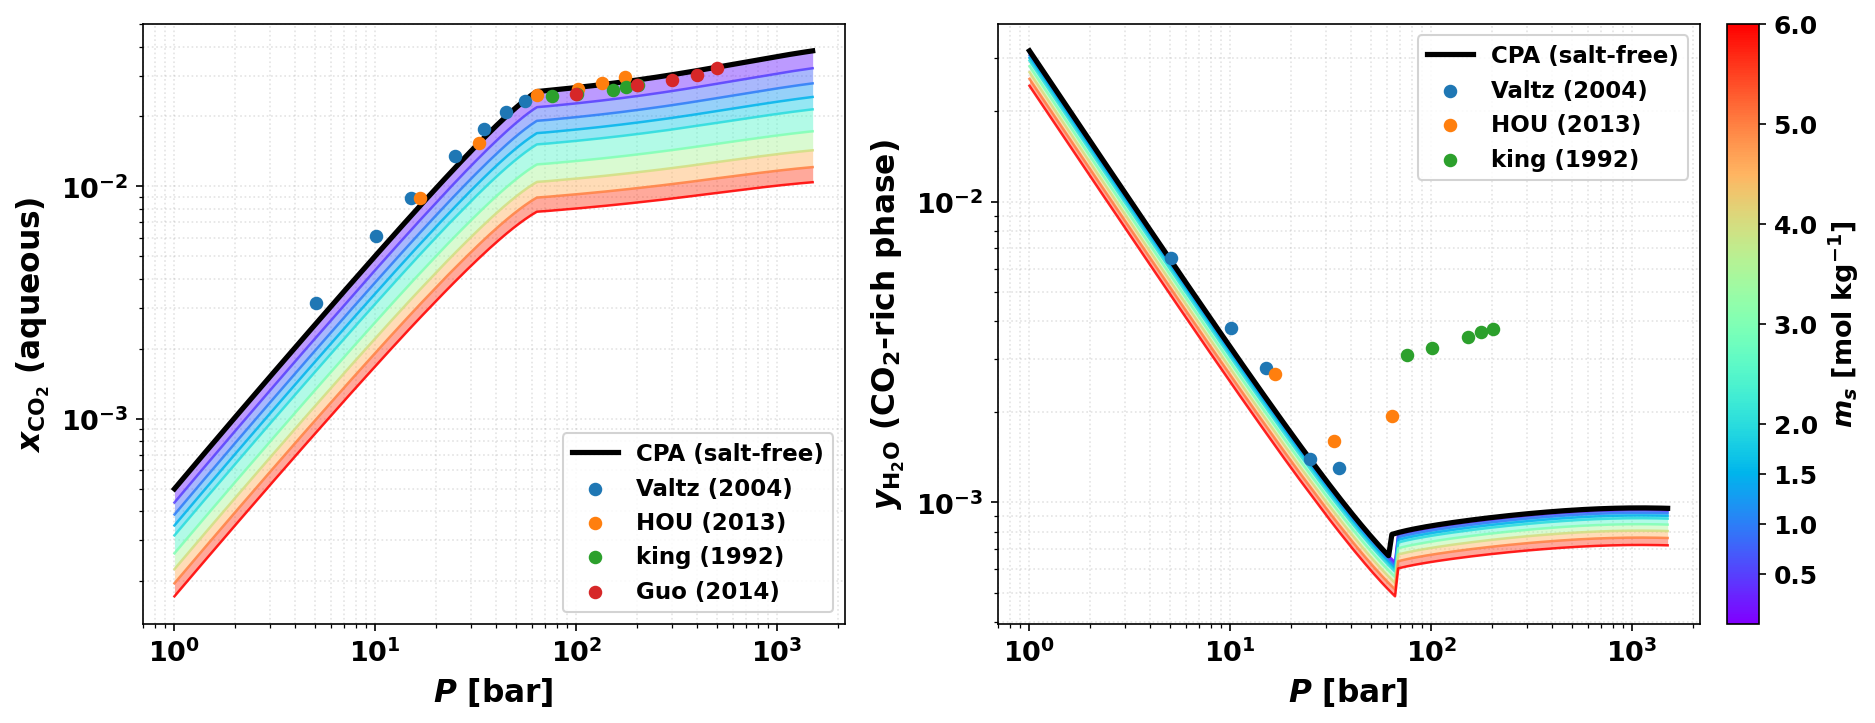
\includegraphics[width=.85\textwidth]{fig_1a.png}\caption{$25\,^\circ$C\,(298\,K)}\end{subfigure}\\[6pt]
  \begin{subfigure}[t]{\textwidth}\centering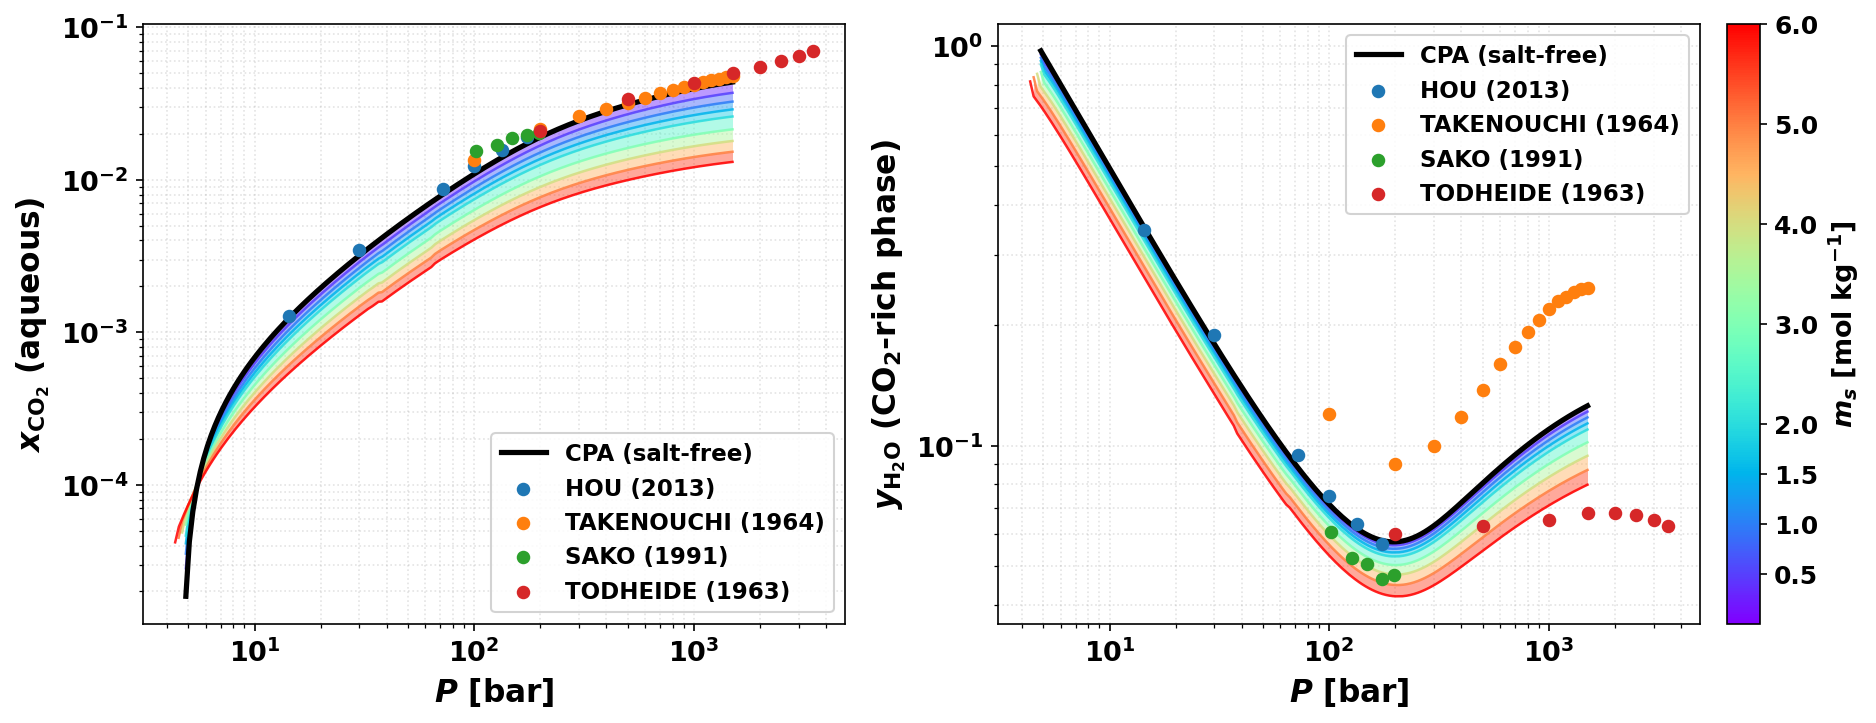
\includegraphics[width=.85\textwidth]{fig_1d.png}\caption{$150\,^\circ$C\,(423\,K)}\end{subfigure}\\[6pt]
  \begin{subfigure}[t]{\textwidth}\centering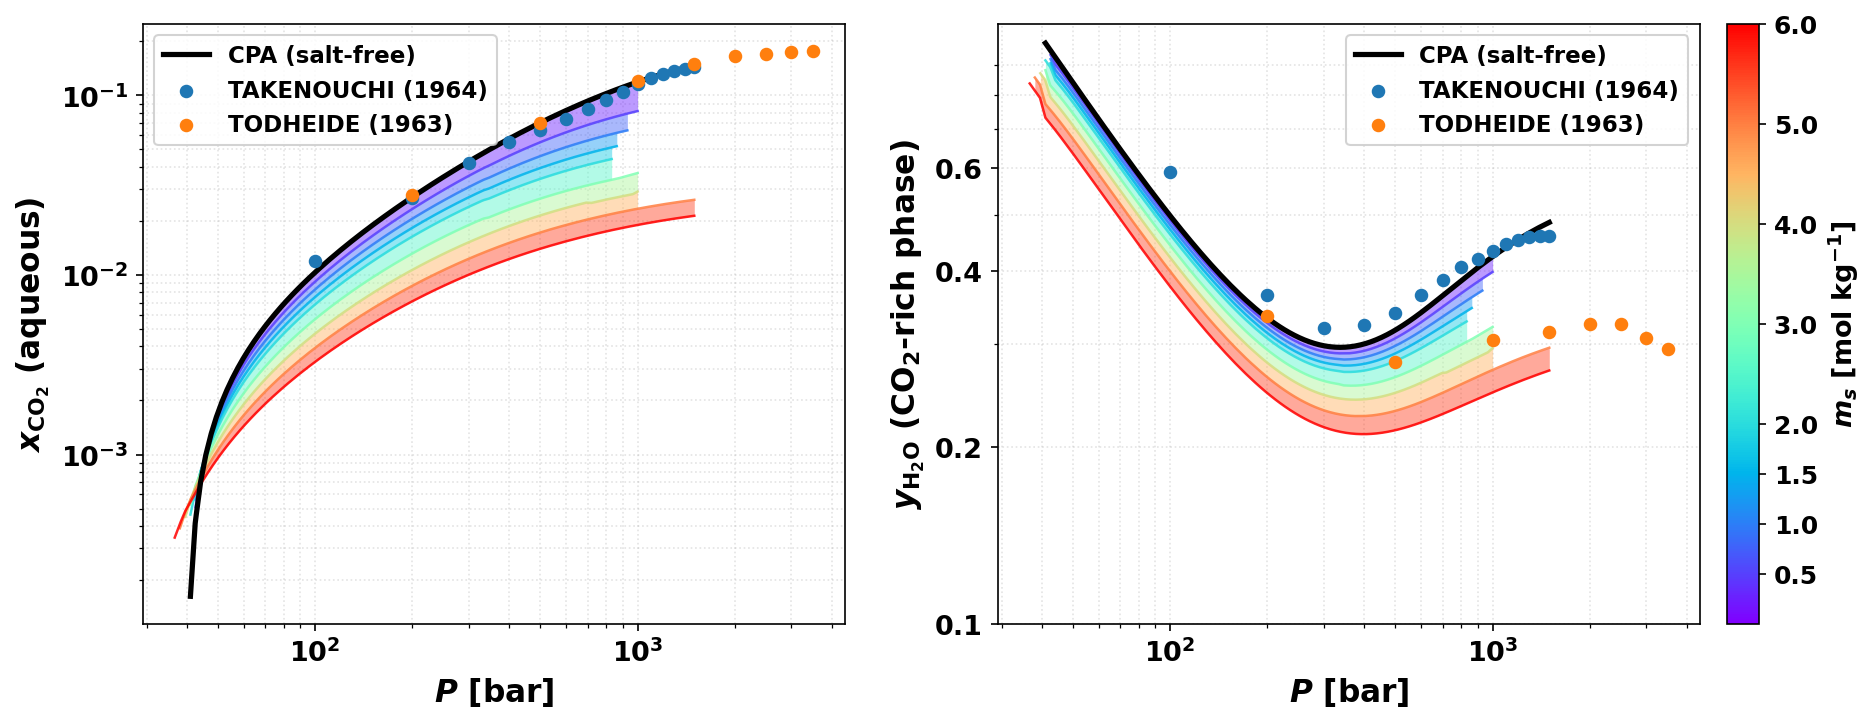
\includegraphics[width=.85\textwidth]{fig_1f.png}\caption{$250\,^\circ$C\,(523\,K)}\end{subfigure}
  \caption{CO$_2$ + H$_2$O phase equilibria at three representative temperatures ($25$, $150$, and $250\,^\circ$C).
           Each panel shows the CO$_2$ mole fraction in the aqueous phase ($x_{\text{CO}_2}$, left sub-panel)
           and the H$_2$O mole fraction in the CO$_2$-rich phase ($y_{\text{H}_2\text{O}}$, right sub-panel)
           vs.\ pressure.
           Open symbols: experimental data \citep{Coelho2025}; black solid line: CPA (salt-free);
           rainbow-colored filled bands: eCPA predictions spanning NaCl molalities
           $m_s = 0$--$6$\,mol\,kg$^{-1}$ (filled between consecutive molality contours;
           violet $\approx 0$, red $= 6$\,mol\,kg$^{-1}$), with discrete eCPA curves overlaid.
           Results for the remaining 32 temperatures are shown in Fig.~S1.}
  \label{fig:co2h2o_Tpanel}
\end{figure}

A cross-reference consistency analysis (Fig.~S7) further reveals
that the $y_{\text{H}_2\text{O}}$ data of \citet{King1992} are physically suspect:
the reported water content in the CO$_2$-rich phase \emph{increases} with pressure above
the CO$_2$ saturation pressure, contradicting thermodynamic expectations and the measurements
of \citet{Meyer2015} at overlapping conditions.
After excluding flagged outlier references (92 of 631 points, see
Fig.~S7), the overall $y_{\text{H}_2\text{O}}$ AARE decreases from
24.4\% to 17.4\%.


\begin{table}[H]
  \centering
  \caption{VLE accuracy metrics for the CO$_2$ + H$_2$O binary by condition regime.
           AARE: average absolute relative error; AAE: average absolute error (mol\%).
           CPA and eCPA ($m_s = 10^{-4}$) give identical results for this salt-free system;
           only eCPA values are shown.
           ``Excl.\ outliers'' removes references flagged by cross-reference consistency
           (see text).}
  \label{tab:co2h2o_metrics}
  \begin{tabular}{lrrrrrr}
    \toprule
    & \multicolumn{3}{c}{$x_{\text{CO}_2}$ (aqueous)} & \multicolumn{3}{c}{$y_{\text{H}_2\text{O}}$ (CO$_2$-rich)} \\
    \cmidrule(lr){2-4} \cmidrule(lr){5-7}
    Regime & $N$ & AARE & AAE & $N$ & AARE & AAE \\
    \midrule
    All data                          & 560 & 9.6\% & 0.53\,mol\% & 452 & 24.4\% & 3.5\,mol\% \\
    All (excl.\ outliers)             & 468 & 9.3\% & 0.53\,mol\% & 355 & 17.4\% & 3.0\,mol\% \\
    Subsurface                        & 137 & 6.5\% & 0.13\,mol\% & 102 & 25.6\% & 0.68\,mol\% \\
    Extended ($T = 10$--$200\,^\circ$C)    & 362 & 8.9\% & 0.21\,mol\% & 299 & 24.6\% & 1.7\,mol\% \\
    High-$T$ ($T \geq 260\,^\circ$C)        & 129 & 10.1\% & 1.6\,mol\% & 111 & 15.9\% & 8.0\,mol\% \\
    High-$P$ ($P > 1500$\,bar)        & 27  & 18.4\% & 2.9\,mol\% & 27  & 78.0\% & 15.0\,mol\% \\
    \bottomrule
    \multicolumn{7}{l}{\footnotesize Subsurface: $T = 30$--$150\,^\circ$C, $P = 50$--$600$\,bar.} \\
  \end{tabular}
\end{table}

These model errors should be interpreted in the context of the experimental
uncertainty in the compiled dataset.
Two independent estimates of measurement scatter can be obtained directly from the data.
First, at the 76 ($T$, $P$) conditions where at least two independent references overlap
(matched within $\pm 2.5$\,bar), the coefficient of variation between reported values
averages 4.0\% for $x_{\text{CO}_2}$ and 11.1\% for $y_{\text{H}_2\text{O}}$.
Second, the Gasser--Sroka--Jennen-Steinmetz (GSJS) difference-based variance
estimator \citep{Gasser1986}, which estimates measurement noise from the
scatter of consecutive data points around a locally interpolated trend within each
isothermal series, yields a median relative noise of 2.4\% for $x_{\text{CO}_2}$ and
4.7\% for $y_{\text{H}_2\text{O}}$.
Taken together, these estimates suggest an intrinsic experimental uncertainty
of roughly 2--4\% for $x_{\text{CO}_2}$ and 5--11\% for $y_{\text{H}_2\text{O}}$,
so the model AARE of 6.5\% (subsurface) to 9.6\% (global) for $x_{\text{CO}_2}$
are close to the measurement noise.

Moreover, relative errors can be misleading when mole fractions span several orders of
magnitude: a 35\% AARE for $y_{\text{H}_2\text{O}} < 0.005$ (101 points) corresponds to an
average absolute error (AAE) of only 0.1 mol\%---negligible for reservoir
simulation.  Across all data, the AAE is 0.53 mol\% for $x_{\text{CO}_2}$ and
3.5 mol\% for $y_{\text{H}_2\text{O}}$; under subsurface conditions these drop to
0.13 and 0.68 mol\%, respectively.






\subsection{CO$_2$ + NaCl brine}
\label{sec:co2nacl}

\begin{figure}[H]
  \centering
  \newcommand{\snw}{0.47\textwidth}%
  \begin{subfigure}[t]{\snw}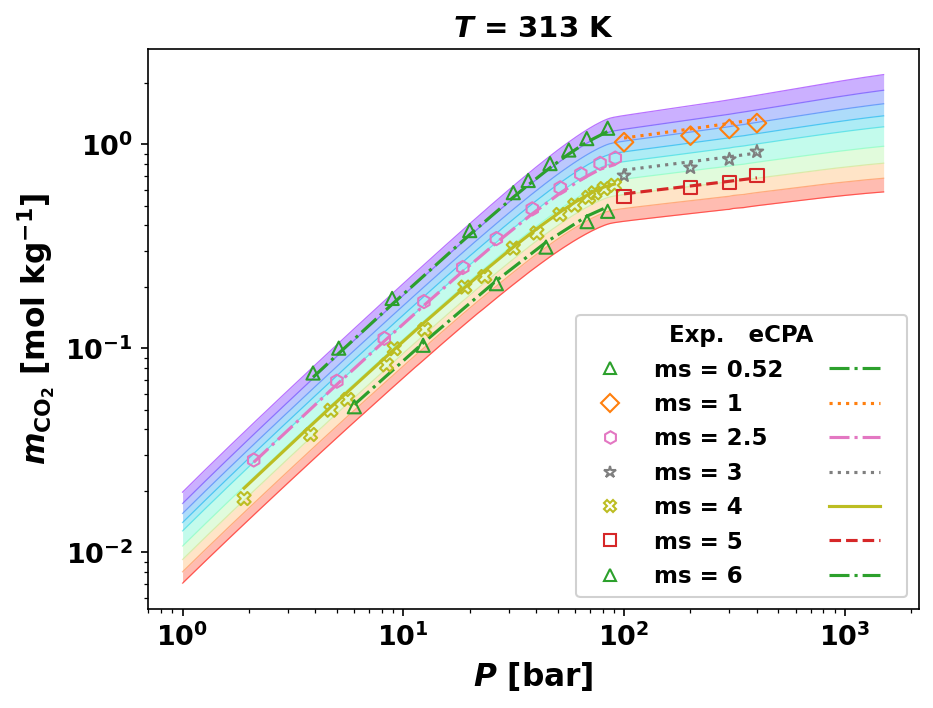
\includegraphics[width=\textwidth]{fig_2b.png}\caption{$40\,^\circ$C}\end{subfigure}\hfill
  \begin{subfigure}[t]{\snw}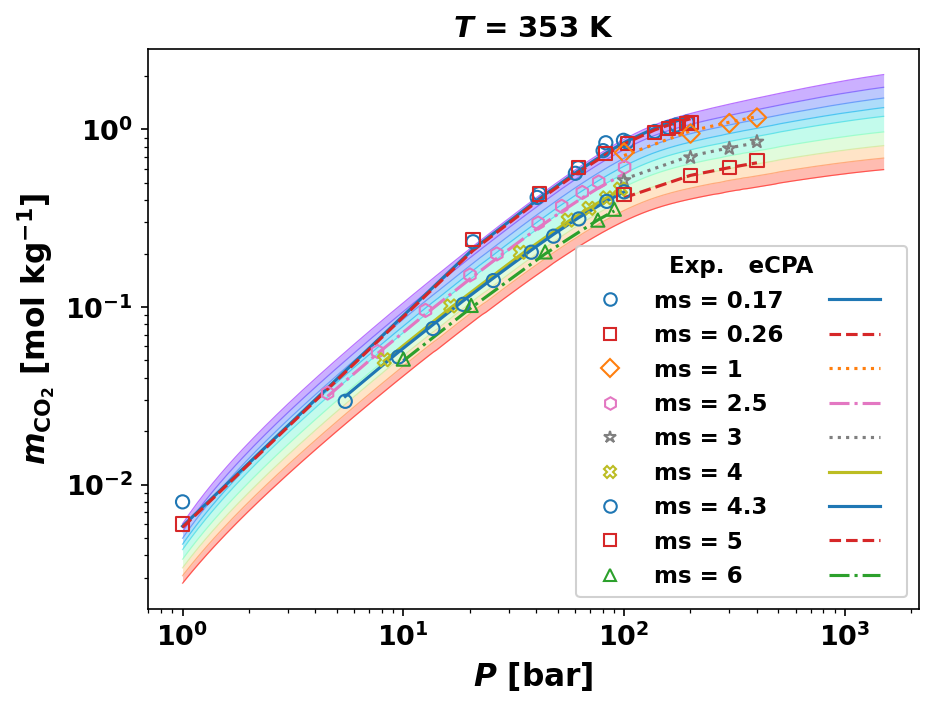
\includegraphics[width=\textwidth]{fig_2c.png}\caption{$80\,^\circ$C}\end{subfigure}\\[6pt]
  \begin{subfigure}[t]{\snw}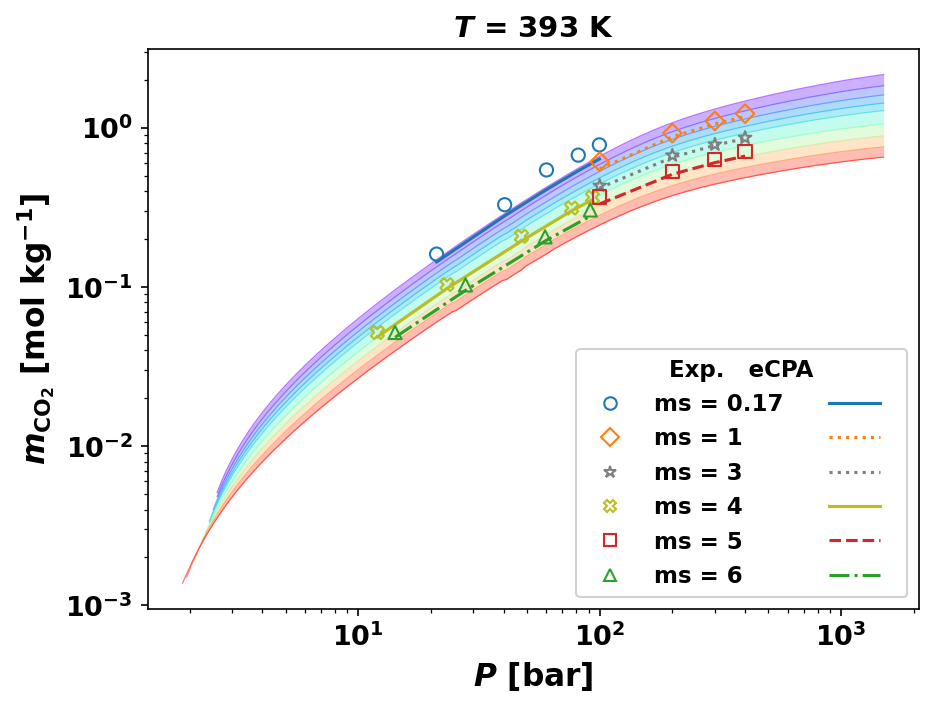
\includegraphics[width=\textwidth]{fig_2d.png}\caption{$120\,^\circ$C}\end{subfigure}\hfill
  \begin{subfigure}[t]{\snw}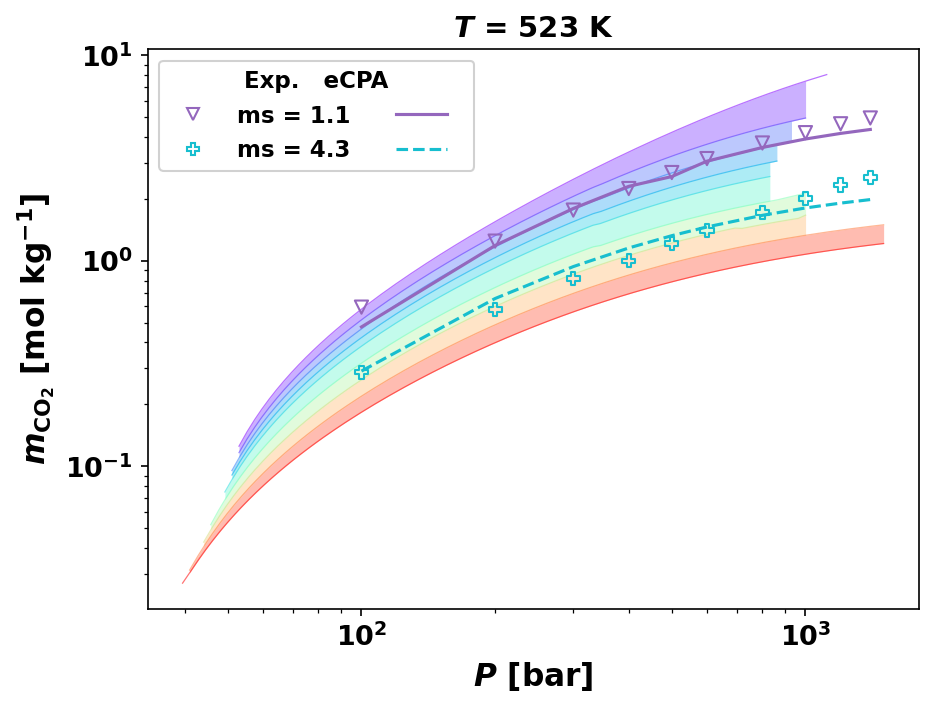
\includegraphics[width=\textwidth]{fig_2f.png}\caption{$250\,^\circ$C}\end{subfigure}
  \caption{CO$_2$ solubility in NaCl brine at four representative temperatures ($40$, $80$, $120$, and $250\,^\circ$C).
           Each panel shows CO$_2$ molality $m_{\text{CO}_2}$ [mol\,kg$^{-1}$] vs.\ pressure (log--log).
           Open symbols: experimental data \citep{Guo2015, Rumpf1994, Kiepe2002,
           Nighswander1989, Bando2003, Liu2021, Takenouchi1965}; discrete lines
           with markers: eCPA at the experimental NaCl molalities.
           Rainbow-colored background bands: continuous eCPA predictions spanning
           $m_s = 0$--$6$\,mol\,kg$^{-1}$ (color scale as in Fig.~\ref{fig:co2h2o_Tpanel}:
           violet $\approx 0$, red $= 6$\,mol\,kg$^{-1}$).
           Temperatures with additional CO$_2$-rich phase data ($y_{\text{CO}_2}$) are shown separately
           in Fig.~\ref{fig:co2nacl_2panel}; all 18 temperatures in Figs.~S2 and~S3.}
  \label{fig:co2nacl_Tpanel}
\end{figure}


Figure~\ref{fig:co2h2o_Tpanel} also illustrates the effect of brine salinity on the equilibrium compositions by including predictions for the full molality range considered in this work. 
We further validate the eCPA ternary flash against all available experimental data from the
literature \citep{Guo2015, Rumpf1994, Koschel2006, Kiepe2002, Takenouchi1965,
Chabab2020, Messabeb2016, Hou2013, Yan2011, Zhao2015,
Bando2003, Nighswander1989, Liu2021, Liu2011b, Savary2012},
spanning $T = 5$--$450\,^\circ$C, $P = 1$--$1400$\,bar, and
$m_s = 0.17$--$6.0$\,mol\,kg$^{-1}$ NaCl (708 experimental data points in total).
Two types of measurements are compared: CO$_2$ solubility in the aqueous
phase and the CO$_2$ mole fraction in the CO$_2$-rich phase
($y_{\text{CO}_2}$).
Aqueous-phase solubility is reported differently by different sources:
as CO$_2$ molality ($m_{\text{CO}_2}$ [mol\,kg$^{-1}$]), or as the mole fraction
on a NaCl-free basis
($x_{\text{CO}_2}^{\text{sf}} = x_{\text{CO}_2}/(x_{\text{CO}_2}+x_{\text{H}_2\text{O}})$),
where NaCl is excluded from the denominator.
The latter is a reporting convention used by some authors and describes
the same physical quantity as $m_{\text{CO}_2}$; it is converted to molality via
$m_{\text{CO}_2} = x_{\text{CO}_2}^{\text{sf}}/[(1-x_{\text{CO}_2}^{\text{sf}})M_w]$
before comparison.






All experimental results and eCPA predictions are illustrated in Figs.~\ref{fig:co2nacl_Tpanel}, \ref{fig:co2nacl_2panel}, S2, and~S3.

Table~\ref{tab:co2nacl_metrics} shows the accuracy breakdown.
689 of 708 points converge to a two-phase solution using the K-value SSI warm-started
from the solution table; the model predicts single-phase behavior at 18 points
(particularly at $T \geq 350\,^\circ$C where CO$_2$ + H$_2$O approaches complete
miscibility in the model) and fails to converge at one extreme high-$P$, high-$m_s$
condition, giving an overall two-phase convergence rate of 97.3\%.
The K-value SSI requires a median of 6 outer iterations per converged call.
Overall AARE across all converged points is 6.2\%, with a slight underprediction bias
of $-1.5\%$.
The AARE for $m_{\text{CO}_2}$ across all $T$ and $m_s$ is 6.6\%, in excellent agreement with the 6.9\%
reported by \citet{Coelho2025} using the original eCPA parameterization.
The CO$_2$-rich phase composition $y_{\text{CO}_2}$ is reproduced to within 0.4\% AARE, reflecting the
near-purity of the CO$_2$-rich phase and its weak dependence on salinity.

At hydrothermal temperatures, AARE for $m_{\text{CO}_2}$ rises to 14.0\% at $T = 300\,^\circ$C and
12.8\% at $T = 350\,^\circ$C, reflecting reduced eCPA accuracy at conditions beyond the
conventional reservoir temperature range.
At $T \geq 400\,^\circ$C, the available experimental pressures (300--900\,bar, all from
\citealt{Takenouchi1965}) fall in the region where eCPA predicts single-phase behavior,
suggesting that the CO$_2$ + H$_2$O miscibility gap closes at these extreme conditions
in the model.
Notably, accuracy at the lowest temperatures ($T = 5$--$10\,^\circ$C) is also reduced
(AARE 14--21\%), reflecting the challenge of modeling CO$_2$ solubility very close to
the freezing point where eCPA is not specifically parameterized.
These conditions furthermore fall within the CO$_2$ hydrate stability zone, where solid
CO$_2$ clathrates can form; the eCPA EoS computes fluid-phase VLE only and does not
model hydrate formation explicitly.
Fig.~S4 provides a comprehensive view of the error distribution
across the full $(T, m_s)$ parameter space: accuracy is best at intermediate temperatures
($T = 27$--$227\,^\circ$C) and moderate salinities ($m_s \leq 3$\,mol\,kg$^{-1}$), and degrades
systematically at the boundaries of the validated range.

\begin{figure}[H]
  \centering
  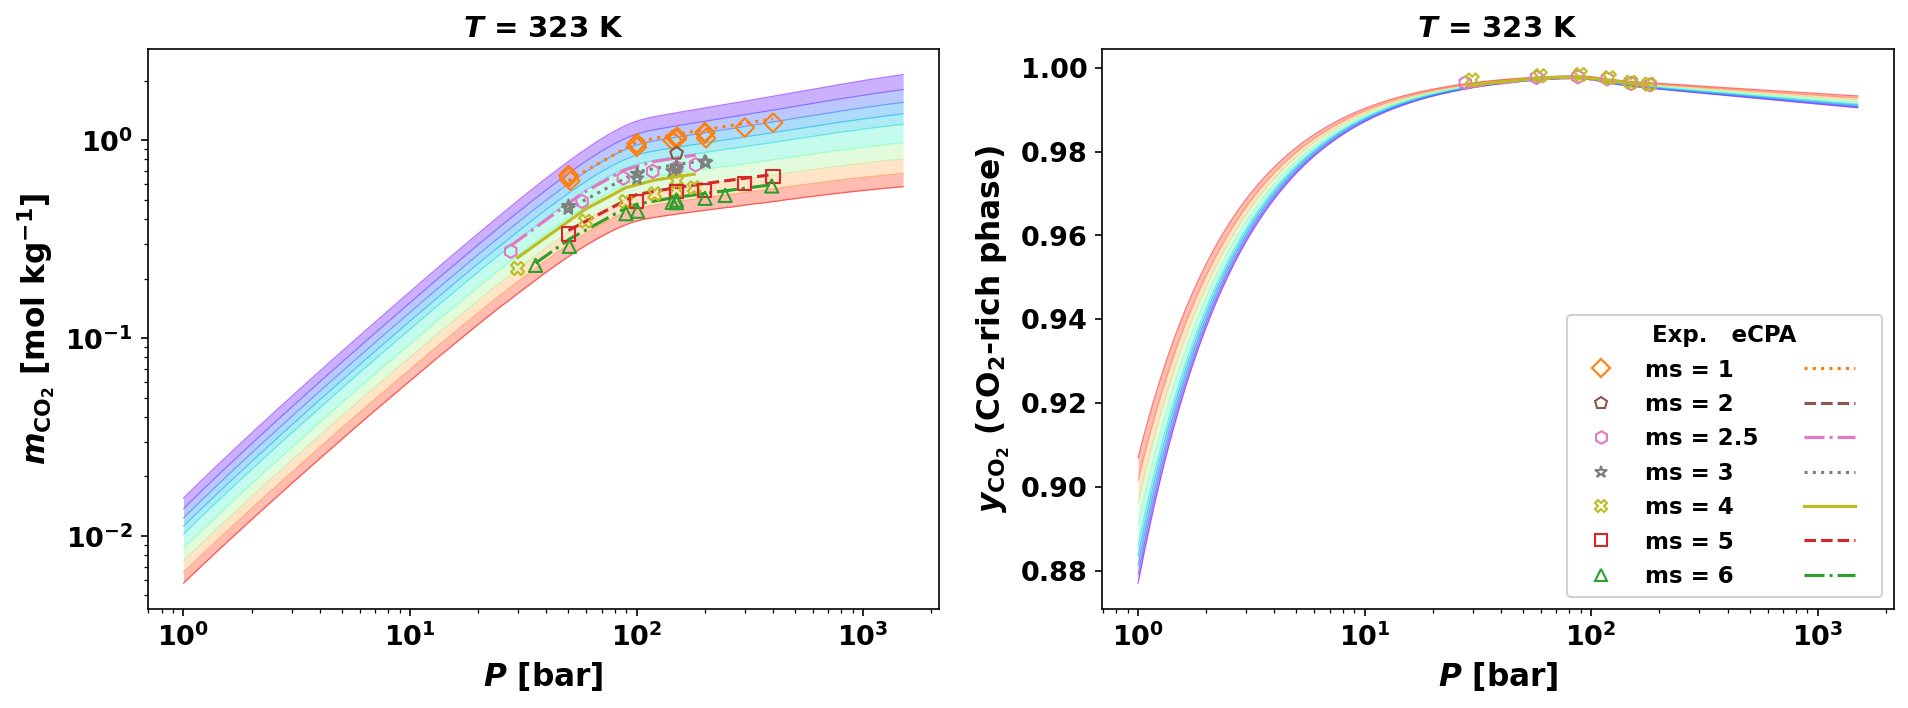
\includegraphics[width=0.9\textwidth]{fig_3a.png}\\[6pt]
  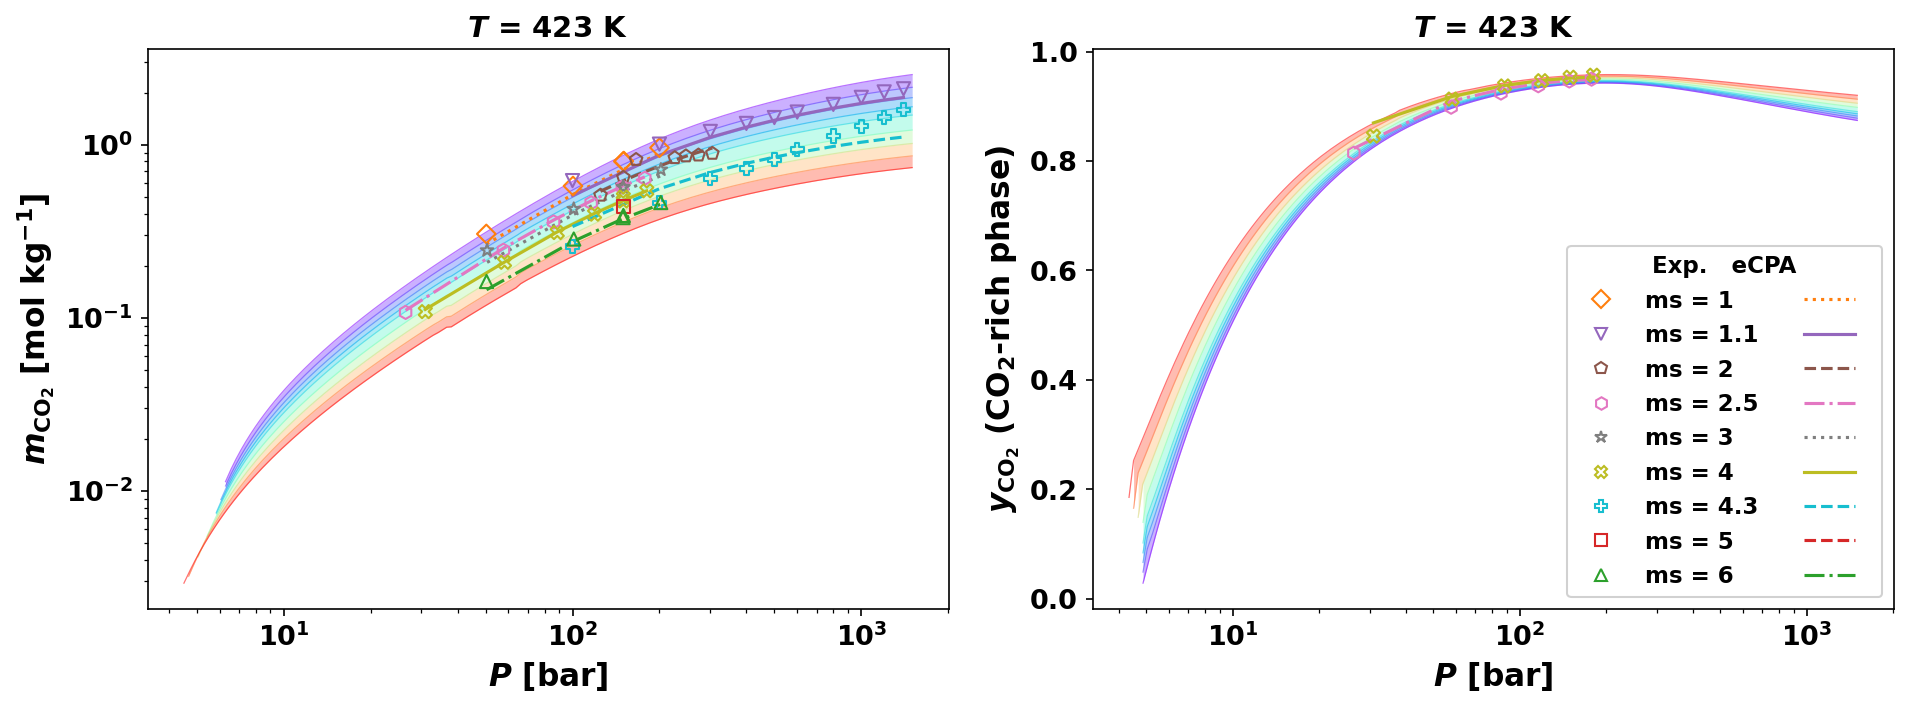
\includegraphics[width=0.9\textwidth]{fig_3c.png}
  \caption{CO$_2$ + NaCl brine phase equilibria at temperatures for which both CO$_2$ molality
           ($m_{\text{CO}_2}$, left panel) and CO$_2$ mole fraction in the CO$_2$-rich phase ($y_{\text{CO}_2}$, right panel)
           data are available: (top) $50\,^\circ$C, (bottom) $150\,^\circ$C
           (see also Fig.~S3 for $100\,^\circ$C).
           Open symbols: experimental data \citep{Bando2003, Chabab2020, Guo2015,
           Hou2013, Koschel2006, Liu2021, Messabeb2016, Savary2012, Takenouchi1965,
           Yan2011, Zhao2015}; discrete lines with markers: eCPA at the
           experimental NaCl molalities.
           Rainbow-colored background bands: continuous eCPA predictions across
           $m_s = 0$--$6$\,mol\,kg$^{-1}$ (color scale as in Fig.~\ref{fig:co2h2o_Tpanel}).}
  \label{fig:co2nacl_2panel}
\end{figure}



\begin{table}[H]
  \centering
  \caption{VLE accuracy metrics for CO$_2$ + NaCl brine ($T = 5$--$450\,^\circ$C,
           $m_s = 0.17$--$6.0$\,mol\,kg$^{-1}$, 708 data points total,
           689 two-phase converged). Bias $= \langle(\hat{y} - y)/y\rangle$.}
  \label{tab:co2nacl_metrics}
  \begin{tabular}{lrrr}
    \toprule
    Quantity & $N$ & AARE (\%) & Bias (\%) \\
    \midrule
    $m_{\text{CO}_2}$ [mol\,kg$^{-1}$]            & 501 & 6.6 & $-3.3$ \\
    $x_{\text{CO}_2}^{\text{sf}}$ (NaCl-free basis, conv.\ to $m_{\text{CO}_2}$) & 116 & 5.5 & $+2.7$ \\
    $x_{\text{CO}_2}$ [salt-incl.]    &  36 & 8.6 & $+8.6$ \\
    $y_{\text{CO}_2}$                 &  36 & 0.5 & $-0.1$ \\
    \midrule
    All converged           & 689 & 6.2 & $-1.5$ \\
    \bottomrule
  \end{tabular}
\end{table}







\subsection{Flash results as a function of feed composition}
\label{sec:flash_vs_z}

A central motivation for full stability+flash --- rather than straightforward
VLE calculations at a fixed salinity --- arises naturally in reservoir simulation.
When CO$_2$ is injected into a saline aquifer, the reservoir fluid at any given
grid cell can be represented as a mixture of brine (carrying NaCl at feed molality
$m_s$) and varying amounts of injected CO$_2$.
The overall CO$_2$ mole fraction $z_{\rm CO_2}$ in this mixture is the primary degree of freedom,
and stability+flash must be performed to determine the equilibrium state.

As shown in Section~\ref{sec:intro}, in the ternary system the equilibrium molality
$m_s^\mathrm{aq}$ exceeds the feed value because NaCl is concentrated as H$_2$O
partitions into the CO$_2$-rich phase; quantitatively (from Eq.~\ref{eq:msaq_kv}):
\begin{equation*}
  m_s^\mathrm{aq}
    = m_s
      \,\frac{(1-\beta)\,x_{\mathrm{H_2O}}+\beta\,y_{\mathrm{H_2O}}}
             {(1-\beta)\,x_{\mathrm{H_2O}}}
    = m_s\!\left(1 + \frac{\beta\,y_{\mathrm{H_2O}}}{(1-\beta)\,x_{\mathrm{H_2O}}}\right),
\end{equation*}
where $\beta$ is the CO$_2$-rich molar phase fraction.
Because $\beta\,y_{\mathrm{H_2O}} > 0$ in the two-phase region, $m_s^\mathrm{aq}$
\emph{exceeds} $m_s$, and the excess grows with $z_{\rm CO_2}$ as $\beta$ increases.
This elevated salinity modifies the aqueous-phase fugacity coefficients and in
turn shifts the equilibrium phase compositions --- an effect that cannot be
captured by a VLE table indexed on feed molality alone.

Figure~\ref{fig:flash_vs_z} demonstrates these effects for $P = 200$\,bar,
$m_s = 1.0$\,mol\,kg$^{-1}$ NaCl, and ten isotherms from $27$ to
$252\,^\circ$C (in $25\,^\circ$C increments) over the two-phase feed range $z_{\rm CO_2} = 0.005$--$0.995$.
Panel (a) shows the CO$_2$-rich phase fraction $\beta$, which rises from 0 to 1
across the two-phase window.
Higher temperatures narrow the window because CO$_2$ is less soluble and
H$_2$O more volatile, both effects shrinking the range of $z_{\rm CO_2}$ that sustains
two-phase coexistence.

Panel (b) illustrates the salinity amplification: at the highest isotherm
($T = 252\,^\circ$C) the ratio $m_s^\mathrm{aq}/m_s$ reaches
$\approx 8$ at the high-$z_{\rm CO_2}$ end of the two-phase window, meaning the aqueous
NaCl concentration increases eightfold relative to the injected brine as H$_2$O
partitions into the growing CO$_2$-rich phase.
At lower temperatures the amplification is smaller because less H$_2$O leaves
the aqueous phase at the lower $\beta$ values attained.

Panel (c) shows the resulting CO$_2$ molality in the aqueous phase,
$m_{\text{CO}_2}$ [mol\,kg$^{-1}$].
Despite operating at fixed $(T, P)$, $m_{\text{CO}_2}$ decreases substantially with increasing
$z_{\rm CO_2}$: at $T = 227\,^\circ$C it falls from $\approx 1.1$ to $\approx 0.4$\,mol\,kg$^{-1}$
across the two-phase window.
This is a direct consequence of the salting-out effect --- the elevated
$m_s^\mathrm{aq}$ suppresses CO$_2$ solubility.
A simple VLE lookup at the feed molality $m_s$ would return the
wrong CO$_2$ solubility for all but the dilute-CO$_2$ end of the window.

\begin{figure}[tp]
  \centering
  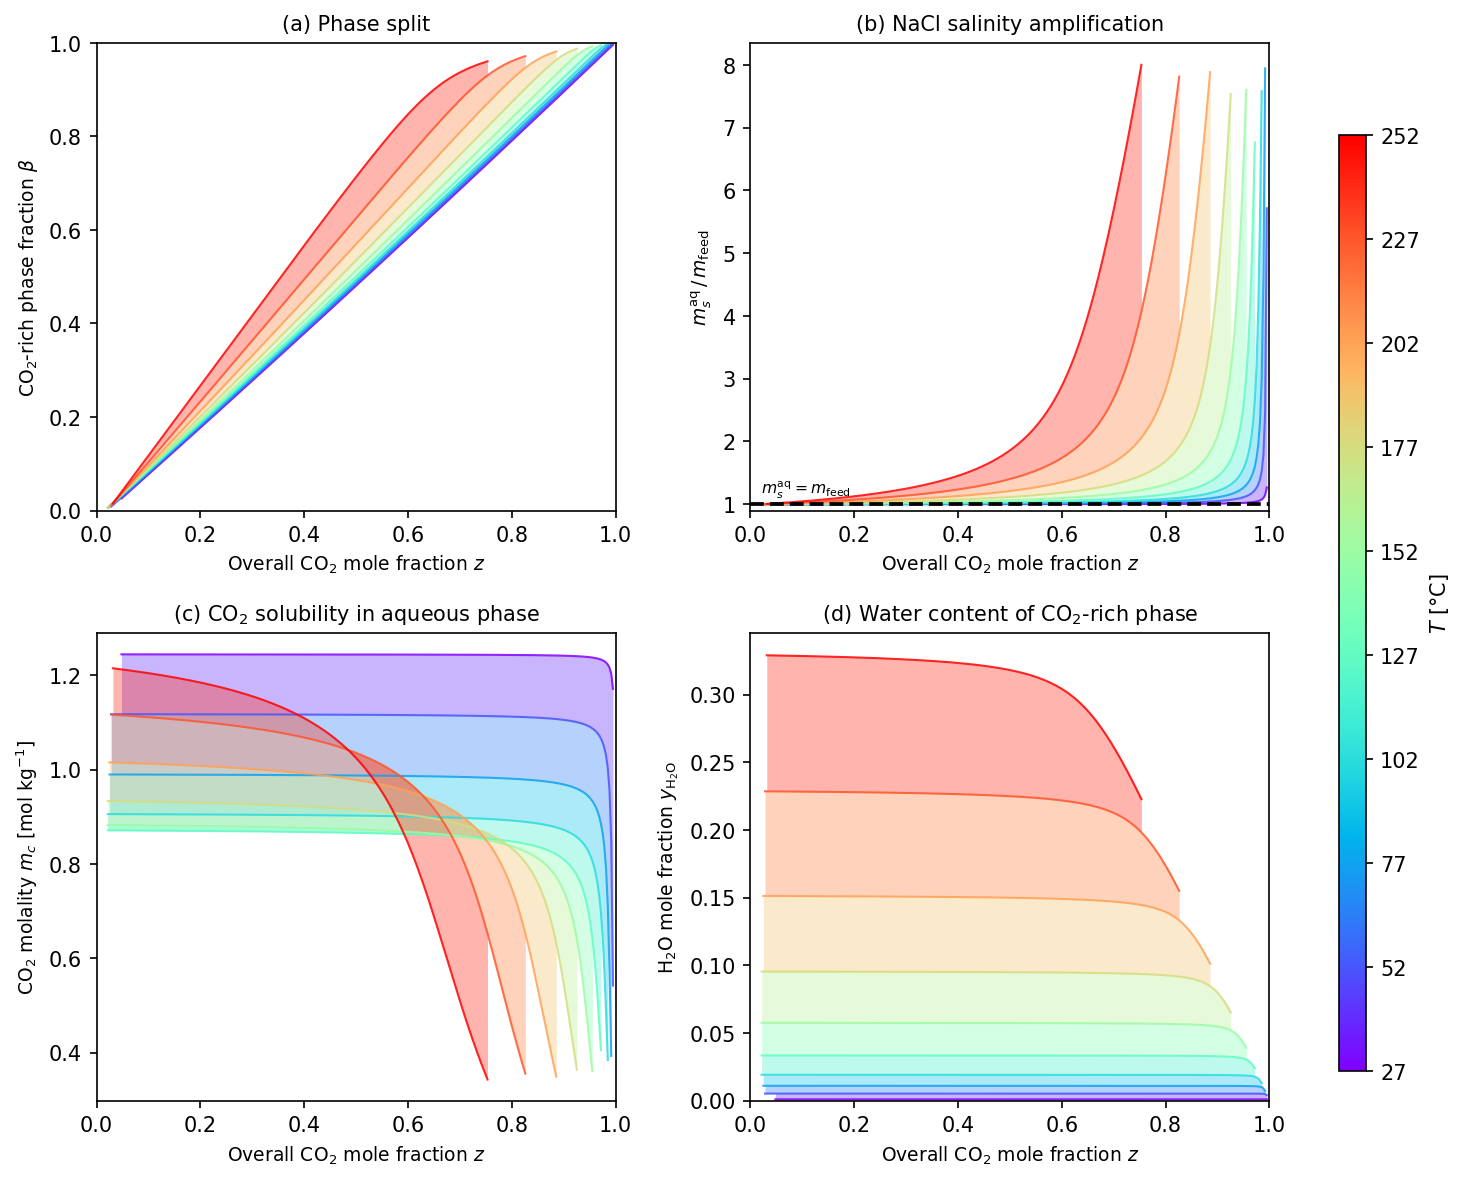
\includegraphics[width=\textwidth]{fig_4.png}
  \caption{eCPA flash results as a function of overall CO$_2$ feed mole fraction $z_{\rm CO_2}$
           at $P = 200$\,bar, feed molality $m_s = 1.0$\,mol\,kg$^{-1}$
           NaCl, and ten isotherms from $27$ to $252\,^\circ$C (violet to red).
           (a) CO$_2$-rich phase fraction $\beta$; the two-phase window narrows
           progressively at higher temperature.
           (b) Ratio of equilibrium aqueous NaCl molality to feed molality,
           $m_s^\mathrm{aq}/m_s$; NaCl concentrates in the aqueous phase
           as H$_2$O partitions to the CO$_2$-rich phase, reaching a factor of ${\sim}8$
           at $T = 252\,^\circ$C and $z_{\rm CO_2} \approx 0.98$.
           (c) CO$_2$ molality $m_{\text{CO}_2}$ in the aqueous phase; the salting-out effect
           driven by the elevated $m_s^\mathrm{aq}$ reduces CO$_2$ solubility
           with increasing $z_{\rm CO_2}$.
           (d) H$_2$O mole fraction $y_{\mathrm{H_2O}}$ in the CO$_2$-rich phase;
           substantial water content at high temperatures (up to ${\sim}30$\,mol\%
           at $252\,^\circ$C) and its strong variation with $z_{\rm CO_2}$ highlight the need
           for full flash rather than a fixed-salinity VLE lookup.}
  \label{fig:flash_vs_z}
\end{figure}

Panel (d) shows the H$_2$O mole fraction in the CO$_2$-rich phase, $y_{\mathrm{H_2O}}$,
and reveals a second consequence of the salting-out chain.
As $z_{\rm CO_2}$ increases, $\beta$ increases and $m_s^\mathrm{aq}$ rises (panel b), which suppresses
CO$_2$ solubility in the aqueous phase (panel c): the aqueous phase can dissolve less CO$_2$,
so proportionally more CO$_2$ remains in the CO$_2$-rich phase and, by molar conservation,
$y_{\mathrm{H_2O}}$ is diluted downward.
At low temperatures this effect is invisible because the baseline water content of
the CO$_2$-rich phase is tiny; at high temperatures, where $y_{\mathrm{H_2O}}$ starts near
$\approx 35$\,mol\%, the same salting-out suppression translates into a large absolute drop
--- falling to $\approx 22$\,mol\% by $z_{\rm CO_2} \approx 0.75$ at $T = 252\,^\circ$C.
This also underscores the importance of accurate modeling of the CO$_2$-rich phase
at elevated temperatures.

Taken together, these results demonstrate that the correct representation of
CO$_2$+brine phase behavior in reservoir models requires a full
stability+flash computation for each cell at each time step, with the
NaCl molality updated self-consistently from the aqueous-phase amount.



\subsection{Aqueous-phase density}
\label{sec:density}

We validate pure-water density by comparing eCPA predictions (with the
temperature-dependent Péneloux shift described in Section~\ref{sec:peneloux})
against the IAPWS-95 international standard \citep{IAPWS2016} — fitted to a
comprehensive body of experimental measurements and valid to 1\,000\,MPa and
1\,273\,K, with a documented uncertainty in liquid-water density of $\pm0.001$--$0.02\%$.
Over 475 liquid/compressed-water conditions spanning
$T = 0$--$350\,^\circ$C and $P = 1$--$2\,000$\,bar, the AARE is \textbf{0.30\%},
with a maximum of 3\% near 350\,$^\circ$C (close to the critical point of water).
For typical subsurface CO$_2$ storage conditions ($T \leq 120\,^\circ$C,
$P = 75$--$600$\,bar), the AARE is \textbf{0.12\%}.
We note that IAPWS-95 is itself a 56-parameter empirical Helmholtz free energy fit
with no molecular basis, optimized specifically to reproduce water data.
Achieving 0.30\% with a physics-based association EoS (CPA/eCPA) is therefore a strong result.
Full details, the parity plot, and the signed-error surface are provided in
Section~S4.1 of the Supplemental Information.


%% ============================================================
\section{Computational Performance}
\label{sec:performance}

\subsection{Flash convergence statistics}
\label{sec:convergence}

\subsubsection{Parameter-space scan for the salt-free CPA binary}

To rigorously evaluate the robustness and efficiency of the accelerated SSI and
multi-guess stability test, we perform a comprehensive parameter-space scan over
$86 \times 18 \times 19 = 29{,}412$ conditions spanning
$T = 0$--$425\,^\circ$C, $P = 1$--$1500$\,bar, and
$z_{\rm CO_2} = 0.001$--$0.999$ (Table~\ref{tab:scan_grid}).
At each $(T, P, z_{\rm CO_2})$ point, we run the stability test with all six initial guesses,
followed by four independent flash strategies:
standard SSI with Wilson K initialization (``Std+Wilson''),
accelerated SSI with Wilson K (``Acc+Wilson''),
accelerated SSI with K from the stability test (``Acc+StabK''),
and the full hierarchical robust algorithm (``Robust'').

\begin{table}[H]
  \centering
  \caption{Parameter-space scan grid for the salt-free CPA binary.}
  \label{tab:scan_grid}
  \begin{tabular}{lrrr}
    \toprule
    Variable & Range & Points & Spacing \\
    \midrule
    $T$ ($^\circ$C)      & 0--425    & 86 & $5\,^\circ$C \\
    $P$ (bar)            & 1--1500   & 18 & semi-log \\
    $z_{\text{CO}_2}$    & 0.001--0.999 & 19 & variable \\
    \midrule
    Total                &           & 29{,}412 & \\
    \bottomrule
  \end{tabular}
\end{table}

Of the 29{,}412 conditions, 19{,}586 (66.6\%) are classified as single-phase by the
stability test and 9{,}825 (33.4\%) as two-phase.
Table~\ref{tab:accel_comparison} compares six flash strategies on the
two-phase subset.
The hierarchical robust algorithm achieves 100\% convergence by combining the
stability-informed K-value initialization with Wilson-K fallback for the
0.3\% of points where the stability K fails to converge.
Only a single point at the extreme corner of the domain ($T = 425\,^\circ$C,
$P = 1500$\,bar, $z_{\text{CO}_2} = 0.995$) produces a spurious instability;
all neighbors are correctly identified as single-phase.


The accelerated SSI reduces the mean iteration count from 25.4 to 13.7
(a 46\% reduction, or $1.9\times$ speedup) compared to standard SSI with the same
Wilson K initialization (Figs.~\ref{fig:scan_summary}a and~S11).
The speedup is most pronounced near the CO$_2$ critical point ($T \approx 31\,^\circ$C,
$P \approx 74$\,bar) and at extreme compositions, where standard SSI requires many
iterations to converge (Fig.~\ref{fig:ssi_heatmap}).
Elevated iteration counts at the lowest temperatures in the scan ($T \lesssim 12\,^\circ$C)
are also noteworthy: these conditions fall within the CO$_2$ hydrate stability zone,
where eCPA --- which computes fluid-phase VLE only --- returns a metastable fluid equilibrium
that may be physically unrealizable.
The additional iterations in this regime likely reflect the difficulty of converging
a fluid-phase flash at conditions where the true equilibrium involves a solid hydrate phase.
Using K-values from the stability test as the flash initial guess provides a further
8\% reduction in iterations (13.7 to 12.6) on average.


\begin{table}[H]
  \centering
  \caption{Comparison of six flash strategies across 9{,}825 two-phase conditions
           from the parameter-space scan ($T = 0$--$425\,^\circ$C, $P = 1$--$1500$\,bar,
           $z_{\rm CO_2} = 0.001$--$0.999$).
           The first four rows use cold-start initialization;
           the fifth and sixth use K-values interpolated from a pre-computed solution table
           extended to $T = 0$--$400\,^\circ$C (99.9\% of two-phase points).
           The sixth row additionally applies Newton polish once $\|\mathbf{g}\| < 10^{-4}$,
           with mean 4.8 SSI and 2.1 Newton iterations per converged call.}
  \label{tab:accel_comparison}
  \begin{tabular}{lrrrr}
    \toprule
    Strategy & Converged & Conv.\ rate & \shortstack{Mean\\iters} & \shortstack{Median\\iters} \\
    \midrule
    Std SSI + Wilson K           & 9{,}756 & 99.3\%  & 25.4 & 17 \\
    Acc SSI + Wilson K           & 9{,}775 & 99.5\%  & 13.7 &  9 \\
    Acc SSI + Stability K        & 9{,}793 & 99.7\%  & 12.6 &  9 \\
    \shortstack[l]{Acc SSI + Stability K\\+ Wilson K} & 9{,}825 & \textbf{100\%} & 13.0 &  9 \\
    \midrule
    Acc SSI + Table K            & 9{,}818 & 99.9\%  &  9.8 &  6 \\
    Acc SSI + Table K + Newton   & 9{,}808 & 99.8\%  &  \textbf{6.9} &  5 \\
    \bottomrule
  \end{tabular}
\end{table}


When a pre-computed solution table is available---as in sequential simulation
where flash solutions from the previous time step or neighboring grid cells
serve as initial guesses---the iteration count drops further to a mean of 9.8
(median~6), a 25\% improvement over the best cold-start strategy.
The table covers $T = 0$--$360\,^\circ$C with $1\,^\circ$C resolution and all practically
relevant pressures ($P = 1$--$2000$\,bar); it captures 99.9\% of the two-phase
scan points, eliminating the Wilson-K fallback for virtually all conditions.
Because the table also pre-classifies each cell as single- or two-phase, the
Michelsen stability test (six guesses, $\approx10$\,ms per guess) can be skipped
for all cells confidently inside the two-phase window, so the dominant cost of a
cold-start stability+flash call ($\approx30\times$ higher wall time) is avoided
in the warm-start regime.
Phase compositions obtained from the two approaches agree to within 1.1\% AARE
for $x_{\text{CO}_2}$ and 3.9\% for $y_{\text{H}_2\text{O}}$, with residual
discrepancies concentrated near the two-phase boundary where both methods are
most sensitive to initial guesses.


\begin{figure}[tp]
  \centering
  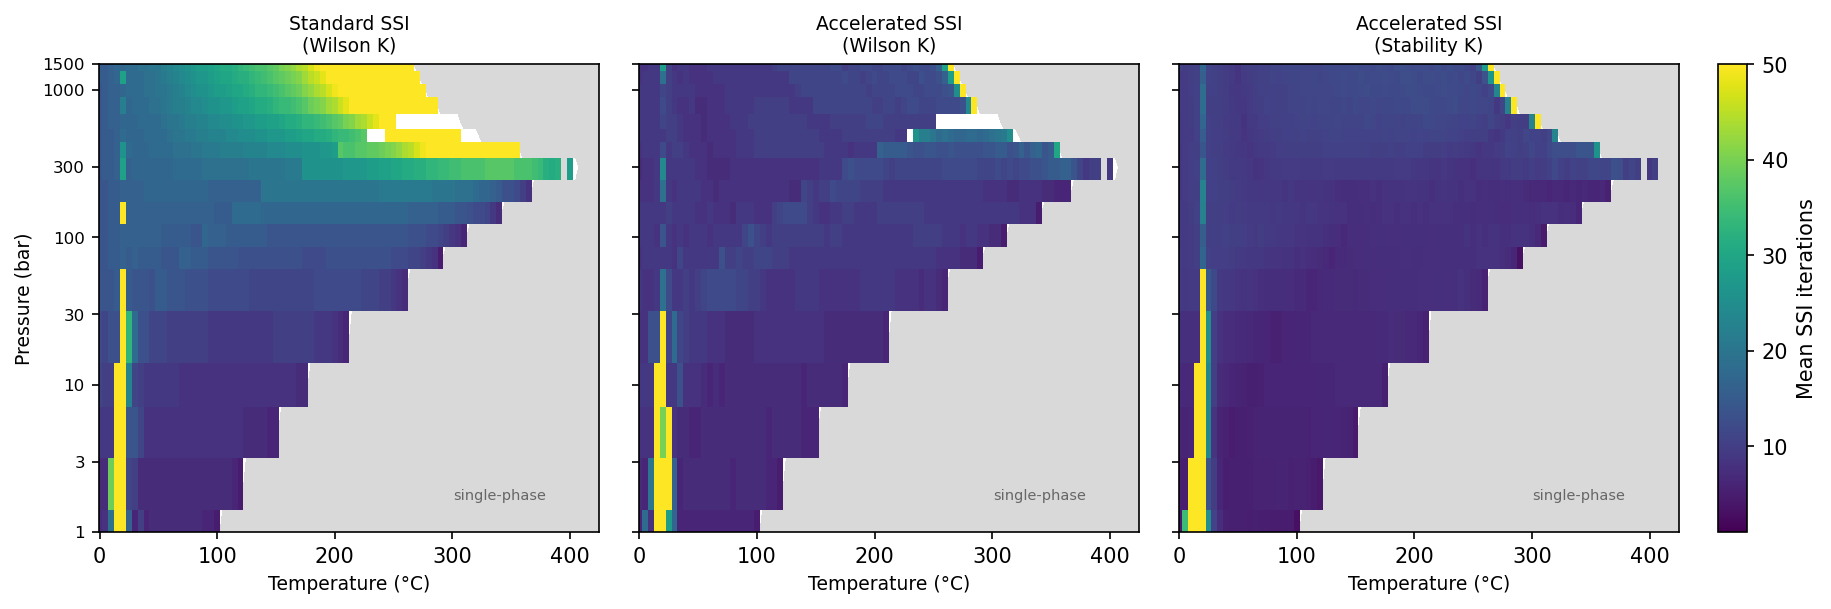
\includegraphics[width=\textwidth]{fig_5.png}
  \caption{Mean SSI iteration count for the salt-free CPA flash, averaged over all
           $z_{\text{CO}_2}$ values (two-phase points only), as a function of $T$ and $P$.
           Left: standard SSI with Wilson K initialization.
           Center: accelerated SSI with Wilson K.
           Right: accelerated SSI with stability-test K.
           The accelerated SSI substantially reduces iteration counts across the
           entire parameter space, with the largest improvements near the CO$_2$
           critical point ($T \approx 31\,^\circ$C, $P \approx 74$\,bar).
           Elevated counts at the lowest temperatures ($T \lesssim 12\,^\circ$C) also
           reflect conditions within the CO$_2$ hydrate stability zone, where eCPA
           computes a metastable fluid-phase equilibrium.}
  \label{fig:ssi_heatmap}
\end{figure}

Adding Newton polish (Table~\ref{tab:accel_comparison}, bottom row) reduces the
mean count further to 6.9 (4.8 SSI + 2.1 Newton), a 29\% improvement over
table-warm-started SSI alone and a 73\% reduction from the standard cold-start.
Newton polish is triggered at 85.6\% of points; the remaining 14.4\% converge
in fewer than $\tau_\text{switch} = 10^{-4}$ SSI steps and need no Newton
correction.
In the near-CO$_2$-critical region ($T \approx 7$--$57\,^\circ$C) the Newton step
can temporarily diverge; the solver then reverts to the pre-Newton SSI state
and continues, so no convergence is lost in that region.
The iteration breakdown and wall-time ratio across the full $(T, P)$ parameter
space are shown in Fig.~S10.



\begin{figure}[H]
  \centering
  \begin{subfigure}[t]{0.48\textwidth}
    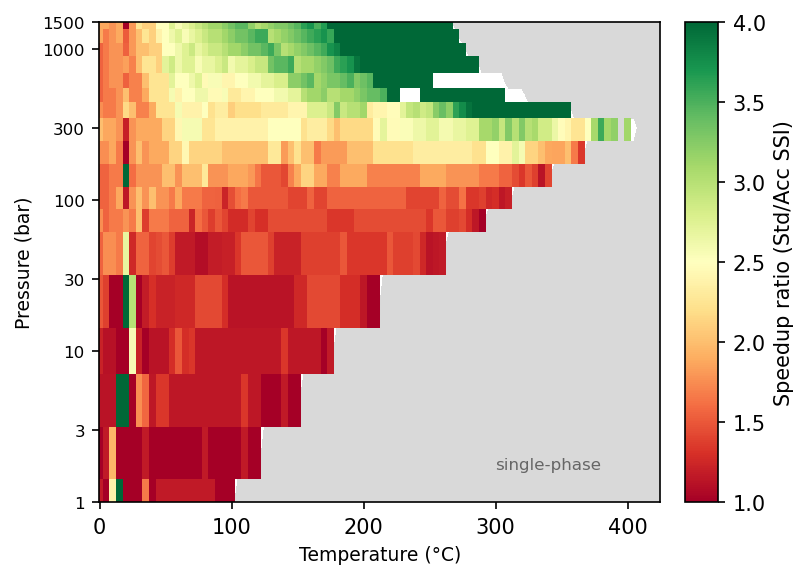
\includegraphics[width=\textwidth]{fig_6a.png}
    \caption{Iteration speedup ratio (standard/accelerated SSI)}
    \label{fig:speedup_ratio}
  \end{subfigure}\hfill
  \begin{subfigure}[t]{0.48\textwidth}
    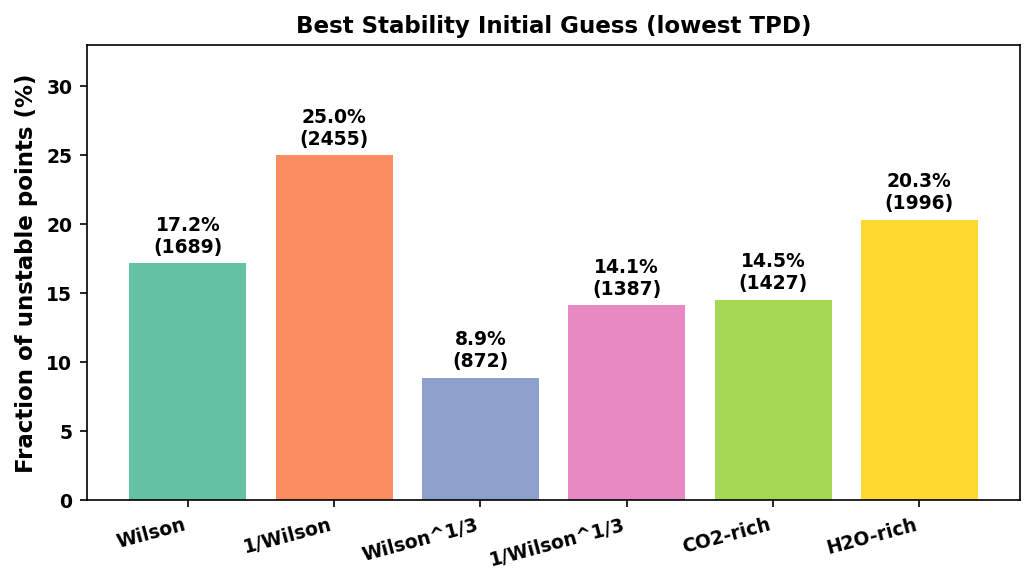
\includegraphics[width=\textwidth]{fig_6b.png}
    \caption{Distribution of best stability initial guess}
    \label{fig:stability_best_trial}
  \end{subfigure}
  \caption{(a) Iteration speedup from accelerated SSI, averaged over $z_{\rm CO_2}$ (two-phase only).
           The speedup exceeds 2$\times$ across most of the parameter space and reaches
           3--4$\times$ near the critical region.
           (b) Distribution of the initial guess that found the lowest TPD across all
           9{,}825 unstable points. No single guess dominates: each of the six trials
           is the best for 9--25\% of conditions, demonstrating the importance of multiple
           initial guesses for robust stability testing.}
  \label{fig:scan_summary}
\end{figure}

Figure~\ref{fig:stability_best_trial} shows that all six stability initial guesses
contribute materially: Wilson is best for 17.2\% of unstable points, inverse Wilson for
25.0\%, H$_2$O-rich for 20.3\%, CO$_2$-rich for 14.5\%, inverse cube-root for 14.1\%, and
cube-root Wilson for 8.9\%.
While the first two guesses (Wilson and inverse Wilson) can detect instability (TPD\,$< 0$)
for 99.8\% of conditions, they locate the \emph{most negative} TPD---and thus the best
K-value initialization for the subsequent flash---for only 42.2\%.
All six guesses are required to ensure the optimal K-value initialization across the
full parameter space.

\subsubsection{Convergence statistics for the eCPA ternary flash}
\label{sec:ecpa_scan}

To characterize eCPA flash performance over the full thermodynamic parameter space
relevant to geological CO$_2$ storage and geothermal energy production, we compute the three-dimensional solution table
described in Section~\ref{sec:table}, covering the grid summarized in
Table~\ref{tab:ecpa_scan_grid}.

\begin{table}[H]
  \centering
  \caption{Parameter grid for the eCPA ternary solution table
           (CO$_2$+H$_2$O+NaCl, $361\times100\times14 = 505{,}400$ points).}
  \label{tab:ecpa_scan_grid}
  \begin{tabular}{lll}
    \toprule
    Dimension & Range & Points \\
    \midrule
    Temperature $T$ & $0$--$360\,^\circ$C & 361 ($1\,^\circ$C steps) \\
    Pressure $P$ & 1--2000\,bar & 100 (log-spaced) \\
    NaCl feed molality $m_s$ & 0--6\,mol\,kg$^{-1}$ & 14 \\
    \bottomrule
  \end{tabular}
\end{table}

Each grid point is evaluated with the full hierarchical stability+flash algorithm: the Michelsen
stability test (six trial compositions) is performed first; only genuinely unstable
conditions proceed to the K-value SSI flash.
The CO$_2$ feed fraction $z_{\rm CO_2}$ is not a table dimension; a representative value
$z_{\rm CO_2} = 0.5$ is used for the stability call (K-values and tie-line endpoints are
only weakly $z_{\rm CO_2}$-dependent, as discussed in Section~\ref{sec:table}).
Of the 505{,}400 grid points, 36{,}100 use the CPA sub-model ($m_s = 0$, no
electrostatic terms); the eCPA model covers the remaining 469{,}300 points.

Table~\ref{tab:ecpa_scan_convergence} reports the outcome of all evaluations.
Every grid point is classified---100\% convergence is achieved over the
complete three-dimensional domain.

\begin{table}[H]
  \centering
  \caption{Classification of eCPA flash outcomes over the full 3D solution table
           (505{,}400 total points; 469{,}300 eCPA, 36{,}100 CPA).}
  \label{tab:ecpa_scan_convergence}
  \begin{tabular}{lrl}
    \toprule
    Classification & Count & Description \\
    \midrule
    Two-phase, converged          & 289{,}065 & Valid two-phase split; SSI converged \\
    Single-phase (stable)         & 216{,}335 & Michelsen stability test: no phase split \\
    \midrule
    Total classified              & 505{,}400 & 100\% \\
    \bottomrule
  \end{tabular}
\end{table}

\begin{figure}[tp]
  \centering
  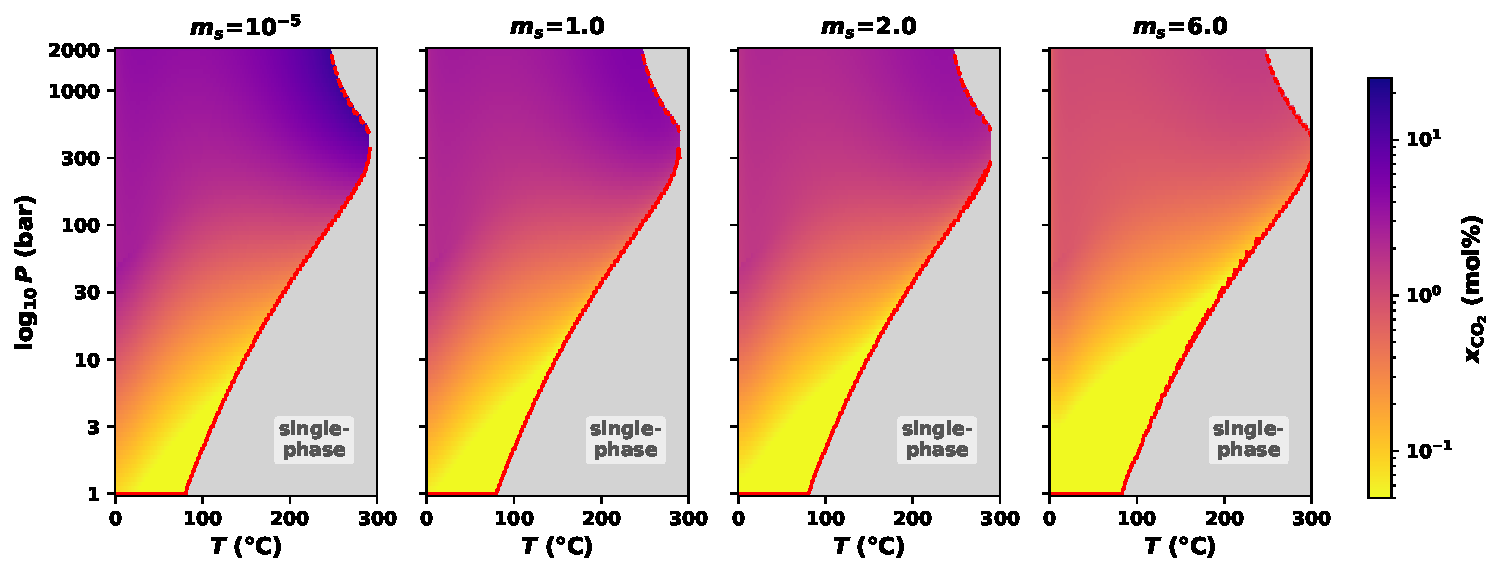
\includegraphics[width=\textwidth]{fig_7.pdf}
  \caption{Equilibrium CO$_2$ mol\% in the aqueous phase ($x_{\text{CO}_2}$)
           over the $T$--$P$ plane at representative feed $z_{\rm CO_2} = 0.5$,
           for six NaCl molalities (columns, $m_s = 0$--$6$\,mol\,kg$^{-1}$).
           The logarithmic color scale spans three orders of magnitude to resolve
           both the dilute near-bubble-point regime and the high-solubility
           hydrothermal limit.
           Grey regions are thermodynamically single-phase at those conditions.
           Red curves mark the phase envelope: the solid line is the dew-point
           boundary (lower pressure limit of the two-phase window) and the dashed
           line is the bubble-point boundary (upper pressure limit).
           The phase boundaries are nearly independent of $m_s$; the salting-out
           effect manifests as a reduction in $x_{\text{CO}_2}$ within the window,
           not as a shift of its extent.}
  \label{fig:ecpa_aq_grid}
\end{figure}

\paragraph{CO$_2$ solubility in the aqueous phase}
Figures~\ref{fig:ecpa_aq_grid} and~\ref{fig:ecpa_c_grid} map $x_{\text{CO}_2}$ and
$y_{\text{H}_2\text{O}}$, respectively, across the full $(T, P)$ domain for six NaCl molalities (and a pure salt-free condition with CPA)
at a representative feed $z_{\rm CO_2} = 0.5$; red curves trace the dew- (solid) and bubble-point (dashed) boundaries,
with the gray region indicating single-phase conditions.
Figure~\ref{fig:ecpa_ssi_heatmap} maps mean flash wall time per call
across the $T$--$P$ plane for all six NaCl molalities, serving as a proxy for
solver effort.
Figure~\ref{fig:ecpa_aq_grid} shows $x_{\text{CO}_2}$ (aqueous phase) over a
logarithmic color scale spanning 0.05--25\,mol\%.
The two-phase window is broad, spanning the full pressure range from 1 to
2000\,bar at most temperatures below $\sim$250\,$^\circ$C, and closes at the highest
temperatures as CO$_2$ and water approach complete miscibility.
Three physically distinct solubility regimes are apparent.
At low temperatures ($T \lesssim 50\,^\circ$C), the CO$_2$-rich phase is a dense
supercritical or liquid-like fluid; solubility is moderate and increases with pressure.
At intermediate temperatures (50--200\,$^\circ$C), solubility passes through a minimum
as the competing effects of pressure and thermal expansion partially cancel.
At high temperatures ($T \gtrsim 250\,^\circ$C), solubility rises sharply because the
aqueous phase increasingly resembles steam; values reach 20--25\,mol\% at the highest
pressures, well into a regime relevant to hydrothermal and geothermal CO$_2$ storage.
Increasing NaCl molality (left to right) reduces CO$_2$ solubility within the
two-phase window---the classical salting-out effect.
The phase boundaries (red curves) are nearly independent of $m_s$: the dew-point
shifts by less than 15\% across the full salinity range,
and the bubble-point (visible only near $T \approx 250\,^\circ$C where it falls below
the 2000\,bar grid ceiling) likewise shows negligible salinity dependence.
The dominant effect of NaCl is therefore a reduction in $x_{\text{CO}_2}$ within the
two-phase window rather than a change in the window's extent.



\paragraph{H$_2$O content of the CO$_2$-rich phase}
Figure~\ref{fig:ecpa_c_grid} shows $y_{\text{H}_2\text{O}}$ (CO$_2$-rich phase) on the same
grid layout.
In sharp contrast to CO$_2$ solubility, the water content of the CO$_2$-rich phase is
controlled almost entirely by temperature: the color field in each panel varies
primarily along the horizontal axis, with near-vertical isopleths.
This reflects the dominant role of the water saturation pressure, which rises steeply
with temperature and sets the water activity in the CO$_2$-rich phase regardless of
pressure or salinity.
At $T = 50\,^\circ$C, $y_{\text{H}_2\text{O}}$ is below 1\,mol\% across
essentially all pressures; by $T = 300\,^\circ$C it reaches 50--70\,mol\%, meaning the
nominal CO$_2$-rich phase is in fact predominantly water vapour.
The effect of NaCl (columns) on $y_{\text{H}_2\text{O}}$ is weak:
the isopleths and the phase envelope (red curves) are essentially unchanged across all
salinity columns, confirming that water content in the CO$_2$-rich phase is set by
temperature alone and is insensitive to brine salinity.

\begin{figure}[tp]
  \centering
  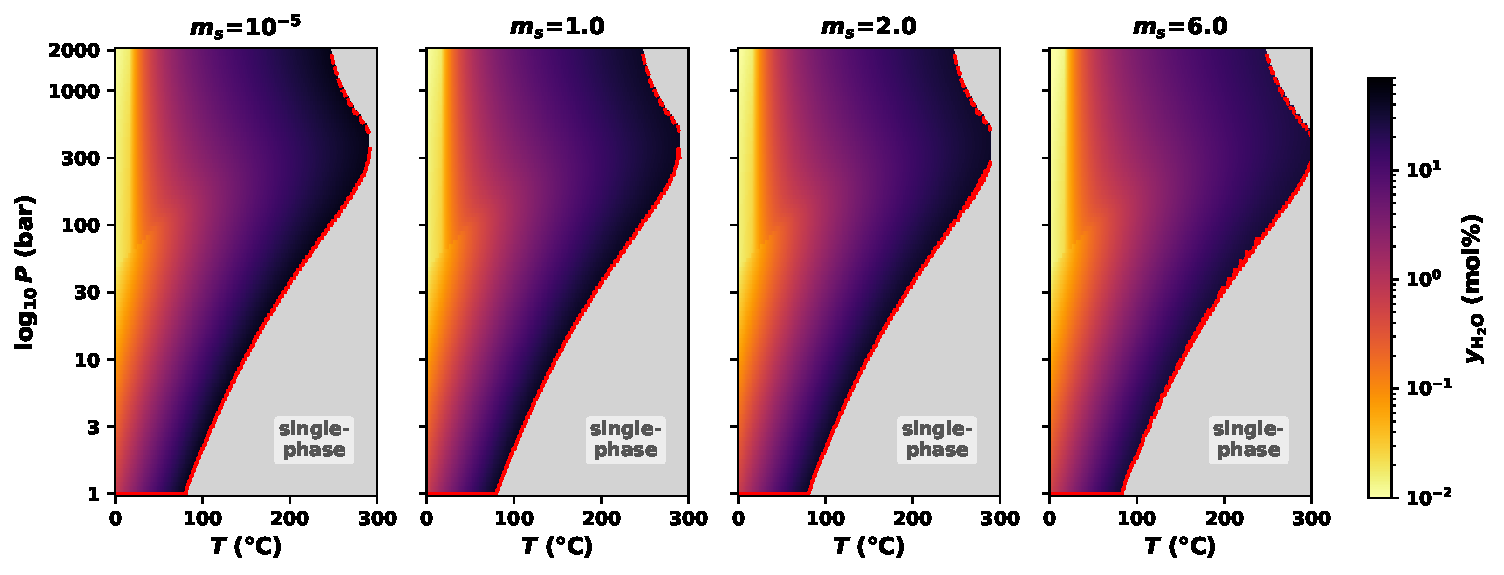
\includegraphics[width=\textwidth]{fig_8.pdf}
  \caption{Equilibrium H$_2$O mol\% in the CO$_2$-rich phase ($y_{\text{H}_2\text{O}}$)
           over the $T$--$P$ plane at representative feed $z_{\rm CO_2} = 0.5$,
           on the same grid as Fig.~\ref{fig:ecpa_aq_grid}.
           Unlike $x_{\text{CO}_2}$, water content in the CO$_2$-rich phase
           is governed almost entirely by temperature (water vapour pressure),
           producing near-vertical isopleths that are nearly independent of
           pressure and NaCl molality.
           Red curves show the phase envelope (solid: dew point; dashed: bubble
           point); their near-identical positions across columns confirm that
           NaCl has negligible influence on the phase boundaries.
           At temperatures above $250\,^\circ$C the CO$_2$-rich phase contains
           more than 25\,mol\% H$_2$O, approaching 70\,mol\% at the highest
           temperatures---a regime relevant to geothermal CO$_2$ storage.}
  \label{fig:ecpa_c_grid}
\end{figure}

\paragraph{Flash wall time}
Figure~\ref{fig:ecpa_ssi_heatmap} maps the mean wall time per eCPA flash call
(table-warm-started K-value SSI) across the $T$--$P$ plane for six NaCl molalities;
gray regions are single-phase.
The $m_s\!=\!0$ (CPA) column is excluded: its cold-start six-trial robust solver
runs at a median of $\sim$215\,ms per call (reported in Table~\ref{tab:convergence}),
which would render uniformly at the colorbar ceiling; the warm-start table applies
equally to CPA.
Wall time serves as a proxy for solver effort.
Times are lowest ($\lesssim 5$\,ms) in the interior of the two-phase region,
where the warm-started SSI converges in 2--3 steps.
Times rise near the phase boundaries---particularly near the bubble point and the
CO$_2$ critical temperature---where K-values approach unity and more iterations
are required.
The pattern is qualitatively similar across all NaCl molalities.

\begin{figure}[tp]
  \centering
  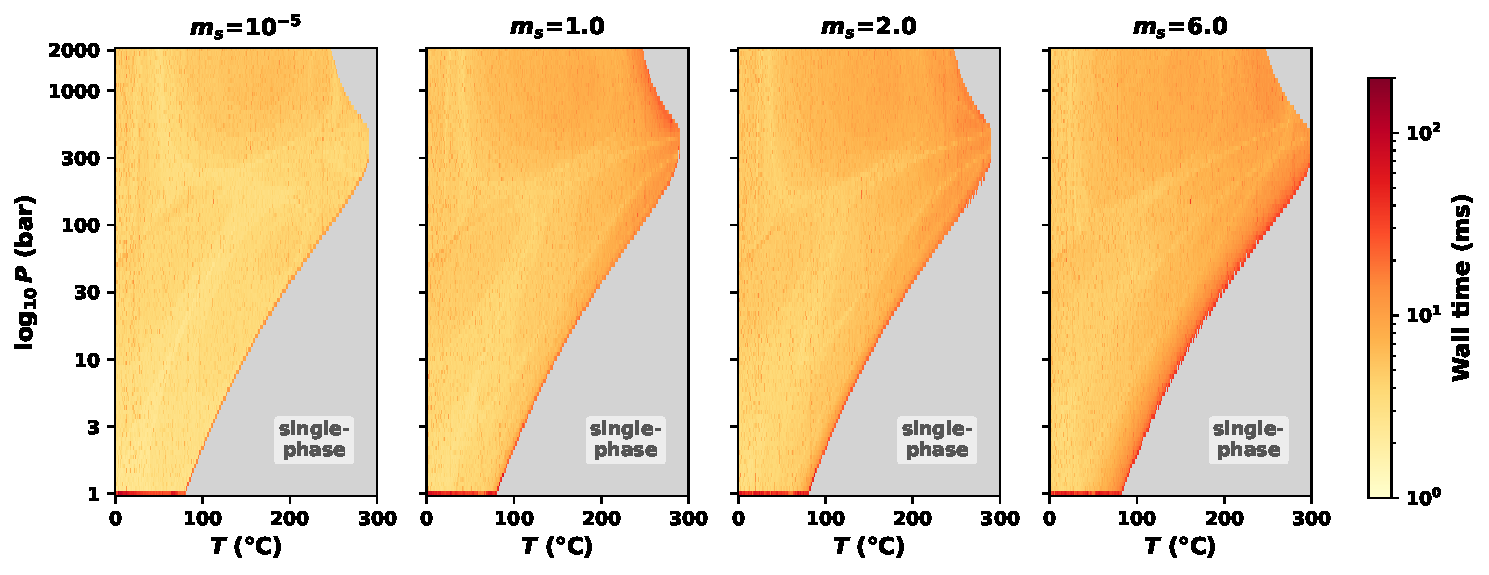
\includegraphics[width=\textwidth]{fig_9.pdf}
  \caption{Mean wall time per flash call (ms) for the eCPA warm-started
           K-value SSI over the $T$--$P$ plane for six NaCl molalities (columns),
           from the 3D scan.
           Gray regions are thermodynamically single-phase.
           The colormap is log-scaled (1--200\,ms).
           Times are lowest in the interior of the two-phase window and highest
           near the phase boundaries where K-values approach unity and more
           SSI iterations are required.
           The $m_s\!=\!0$ (CPA) column is excluded; its cold-start robust solver
           runs at a median of $\sim$215\,ms per call and is reported separately
           in Table~\ref{tab:convergence}.}
  \label{fig:ecpa_ssi_heatmap}
\end{figure}

Table~\ref{tab:convergence} summarizes SSI iteration counts and wall times across the
experimental validation datasets used in Sections~\ref{sec:co2h2o}--\ref{sec:co2nacl}.

\begin{table}[H]
  \centering
  \caption{Flash convergence statistics across the experimental validation datasets.}
  \label{tab:convergence}
  \begin{tabular}{llrrrrl}
    \toprule
    System & Method & $N$ calls & Mean iter & Median & Max & Median time/call \\
    \midrule
    CO$_2$+H$_2$O  & CPA (cold, accel.)   & 29{,}412 &  6.3 &  6 & 272 & $\sim$215\,ms \\
    CO$_2$+H$_2$O  & CPA (warm SSI)       &    626   &  6.2 &  6 &  40 & $\sim$2\,ms   \\
    CO$_2$+H$_2$O  & eCPA (warm SSI, $m_s\!\approx\!0$) &    631   &  5.9 &  6 &  10 & $\sim$2\,ms   \\
    CO$_2$+NaCl    & eCPA (warm SSI)      &    686   &  5.8 &  6 &  16 & $\sim$2\,ms   \\
    \bottomrule
  \end{tabular}
\end{table}
All three warm-start rows use the same solution table and achieve a median of
6 SSI iterations and $\lesssim$2\,ms per call.
The warm-started CPA row directly demonstrates that the $\sim$100$\times$ speedup
over cold-start CPA (row 1) is attributable entirely to the warm-start strategy:
the eCPA model adds electrostatic terms not present in CPA, yet both achieve
comparable wall times when started from a good initial guess.
Among the eCPA rows, the additional salt does not materially increase cost.
Each warm-started SSI step costs only $\sim$0.2\,ms; the solution-table lookup
itself takes $\lesssim$0.05\,ms and contributes negligible overhead.
Convergence is robust across the full validation range.

\subsection{Inner EoS solve efficiency: Newton--Raphson versus cold-start alternatives}
\label{sec:inner_newton_perf}

Each outer SSI iteration requires solving the inner per-phase EoS system.
The two systems — CPA's $(Z, \chi_{\rm H_2O}, \chi_{\rm CO_2})$ and eCPA's $(Z^{\rm aq}, \varepsilon_r, \chi_{\rm H_2O})$
— differ in structure but share the same warm-started Newton--Raphson strategy
described in Sections~\ref{sec:ssi} and~\ref{sec:kv_flash};
the analytical Jacobians are derived in Sections~S3.1 and~S3.2 of the Supplemental Information.
The benchmarks below quantify the advantage of the warm-started Newton solve
over the respective cold-start alternatives, and are distinct from the outer
SSI$+$Newton-polish acceleration discussed in Section~\ref{sec:convergence}
and Fig.~S10.

\paragraph{CPA: $(Z, \chi_{\rm H_2O}, \chi_{\rm CO_2})$ system}
Starting from the previous SSI iterate (typically within 0.5\% of the converged
value), the warm-started Newton solve converges in \textbf{3--4 iterations}
(median~3, maximum~4 across 9{,}825 two-phase conditions).
The cold-start fallback — a 12-point log-spaced scan to bracket the root of $F_1$,
followed by Brent refinement — requires on average 23~residual evaluations
(median~21) per call, equivalent to $\approx$0.38\,ms.
The warm-start Newton solve costs $\approx$0.03\,ms across 128 two-phase conditions
spanning $T = 27$--$227\,^\circ$C and $P = 50$--$800$\,bar:
a \textbf{13$\times$} reduction in inner-solve cost per SSI step.

\paragraph{eCPA: $(Z^{\rm aq}, \varepsilon_r, \chi_{\rm H_2O})$ system}
For the aqueous $3\times 3$ system, a 0.5--1\% warm-start perturbation yields
convergence in \textbf{4--6~iterations} (median~5~at~1\%), with a wall time of
$\approx$0.25\,ms per call.
The cold-start alternative — solving from a heuristic initial guess via a
general-purpose modified-Powell root-finder — requires on average 47~residual
evaluations and costs $\approx$1.5\,ms per call: a \textbf{6$\times$} overhead.

\paragraph{Computational cost of CPA and eCPA versus a cubic EOS}
To quantify the per-iteration overhead of the association terms relative to a plain
cubic EoS, we time each component of a single SSI iteration across 871 two-phase
$(T, P)$ conditions sampled from the CO$_2$--H$_2$O parameter space.
CPA (with the Newton $Z$/$\chi$ solve) is compared against a notional SRK reference
(same EoS parameter computation and fugacity evaluation, but $Z$ found by direct
solution of the cubic and $\chi \equiv 1$).
The per-iteration median wall times were 98\,\textmu{}s (CPA) versus 32\,\textmu{}s
(SRK), a ratio of \textbf{3.1$\times$}.
The EoS-parameter and fugacity-evaluation steps are identical between the two models;
the entire overhead arises in the $Z$/$\chi$ solve, which costs 75\,\textmu{}s
(CPA Newton, two phases) versus 9\,\textmu{}s (SRK direct cubic, two phases).
This factor-of-3 per-iteration cost must be weighed against the additional physics
captured by CPA: accurate partitioning of a self- and cross-associating system over
a wide temperature and pressure range, and (in the full eCPA model) correct salt
activity without empirical brine corrections.

%% ============================================================
\subsection{Simplified versus full flash: accuracy and efficiency}
\label{sec:simplified_perf}

Over 3{,}285 two-phase conditions spanning $T = 10$--$250\,^\circ$C,
$P = 25$--$800$\,bar, and $m_s = 1$--$6$\,mol\,kg$^{-1}$, the simplified flash
reproduces the full K-value SSI result with AARE $< 2\%$ in dissolved CO$_2$ molality
for $T \leq 80\,^\circ$C, rising to 3.2\% at 100\,$^\circ$C and exceeding 5\% above
120\,$^\circ$C as the $y_{\text{H}_2\text{O}} = 0$ assumption deteriorates.
Phase identification agrees with the full flash in 99.7\% of cases.
The accuracy is insensitive to brine salinity: the error is controlled entirely by
temperature.
Contrary to expectation, the mean wall time is essentially identical to the full flash
($0.8\times$ speedup), because Brent root-finding on the 1D fugacity residual requires
$\sim$11 inner Newton evaluations while SSI needs only $\sim$6 outer iterations with at
most two inner solves each.
Full per-temperature statistics, diagnostic figures, and a salinity breakdown are
provided in Section~S4.2 of the Supplemental Information.

%% ============================================================
\section{Reservoir Simulation Demonstration}
\label{sec:simulator}

To confirm that the flash algorithms developed in this work perform reliably under
realistic conditions, we implement them within an isothermal IMPEC compositional
simulator for CO$_2$ injection into heterogeneous 3D saline aquifers.
Across 300 time steps and all 2500 grid cells of a $50\times50$ domain, no flash
failures are recorded in either the salt-free (CPA, $m_s = 0$) or saline
(eCPA, $m_s = 4$\,mol\,kg$^{-1}$) case, confirming 100\% convergence of the
hierarchical stability and flash approach.
The warm-started eCPA flash achieves a throughput of 14{,}270\,calls\,s$^{-1}$ and
the CPA flash 8{,}840\,calls\,s$^{-1}$, with the flash accounting for 80--87\% of
total step cost.
Full details of the numerical scheme, simulation setup, spatial results, and
performance metrics are provided in Section~S6 of the Supplemental Information.


%% ============================================================
\section{Conclusions}
\label{sec:conclusions}

This work presents the first complete phase stability and flash framework built on the
eCPA equation of state of \citet{Coelho2025}, extending it from single-phase property
evaluation to fully converged, production-ready VLE calculations for CO$_2$ + H$_2$O +
NaCl mixtures across reservoir to hydrothermal conditions.

The central algorithmic contribution is the tight integration of four independently
novel elements:
\begin{itemize}
  \item Fast inner Newton--Raphson solvers for the CPA and eCPA root-finding problems,
        based on analytical Jacobians derived in closed form, which reduce the
        per-evaluation overhead to only $\sim$3$\times$ that of a simple cubic EoS.
  \item A hierarchical outer flash algorithm combining Michelsen stability testing with
        six initial guesses, accelerated SSI, and optional Newton polish --- achieving
        100\% convergence over a comprehensive parameter-space scan.
  \item A precomputed three-dimensional $(T, P, m_s)$ solution table that provides warm
        starts reducing flash iterations by a factor of three relative to cold-start SSI.
  \item A simplified flash that exploits the $y_{\text{H}_2\text{O}} \approx 0$
        approximation to reduce the equilibrium problem to a single scalar equation,
        yielding errors below 2\% in dissolved CO$_2$ for $T \leq 80\,^\circ$C at
        essentially the same computational cost.
\end{itemize}
Together, these enable warm-started eCPA flash at throughputs competitive with
conventional cubic-EoS implementations, as demonstrated in a prototype IMPEC reservoir
simulator.

Validation against $>$1100 experimental data points shows AARE of 6.5\% for CO$_2$
solubility under subsurface conditions and 6.6\% for CO$_2$ molality in NaCl brine.
Comparison against the IAPWS-95 international standard over 475 liquid conditions
($T = 0$--$350\,^\circ$C, $P = 1$--$2000$\,bar) with a temperature-dependent Péneloux
volume shift for H$_2$O gives a density AARE of 0.30\% overall and 0.12\% for
subsurface storage conditions.

\section*{Future Work}
\label{sec:future}

A fundamental extension is the generalization to brines containing
multiple salts (e.g.\ NaCl + CaCl$_2$ + MgCl$_2$, as encountered in deep formation
waters).
In the single-salt eCPA framework the NaCl molality provides a single scalar
coupling between phase amounts and phase compositions.
For multi-salt brines the ionic interactions become more complex, and it will likely
be necessary to shift from a molecular-species basis to an ionic basis, treating each
cation and anion as an independent component with its own association and electrostatic
parameters.
Extending the eCPA framework in this direction represents a significant but tractable
step toward a truly general thermodynamic engine for saline CO$_2$ storage.

The algorithms and validation presented here are implemented entirely in Python.
While this facilitates rapid prototyping and transparent benchmarking, it means that
the absolute throughput numbers reported are conservative relative to what a compiled
implementation would achieve.
A natural next step is to integrate the CPA and eCPA flash routines into a
production-level compiled simulator that fully accounts for gravity-driven and
density-driven flow, Fickian diffusion, capillarity, and explicitly resolved discrete
fractures in three-dimensional unstructured grids (e.g.\
\citealt{moortgat2011compositional, moortgat2011three, moortgat2013higher,
moortgat2016mixed, moortgat2018reservoir, solovsky2025efficient, solovsky2026efficient}).
Such an integration will enable high-fidelity simulation of CO$_2$ sequestration
in saline aquifers at reservoir scale.




%% ============================================================
\section*{Acknowledgements}

Abbas Firoozabadi was supported by the member companies of the Reservoir Engineering Research Institute. 

\newpage




%% ============================================================
\section*{Data and Code Availability}

All source code implementing the CPA and eCPA equations of state,
the phase stability and flash algorithms, the solution table construction,
and the reservoir simulator described in this work is freely available at
\url{https://github.com/XXX/ecpa-flash} ($^\ast$upon acceptance of paper).
The repository includes the precomputed three-dimensional solution table,
all experimental VLE data used for validation, and scripts to reproduce
every figure and table in this paper.

%% ============================================================
\section*{Supplementary Information}

The following material is provided as Supplementary Information.

\begin{itemize}
  \item \textbf{Section~S1 (Nomenclature):}
        Complete listing of all mathematical symbols used throughout the paper,
        organized by type (Latin, Greek, subscripts, and superscripts).

  \item \textbf{Section~S2 (EoS Parameters):}
        Tables of pure-component and binary interaction parameters for the CPA/eCPA
        model (Tables~S2--S3), and coefficients for the temperature-dependent
        Péneloux volume shift for H$_2$O (Table~S4; Eq.~S1).

  \item \textbf{Section~S3 (Analytical Jacobians):}
        Closed-form Jacobian matrices for the two inner Newton--Raphson systems:
        the $3\times 3$ CPA system in $(Z,\chi_{\rm H_2O},\chi_{\rm CO_2})$
        and the $3\times 3$ eCPA aqueous-phase system in
        $(Z^{\rm aq},\varepsilon_r,\chi_{\rm H_2O})$ (Eqs.~S2--S29).

  \item \textbf{Section~S4 (Additional Validation Figures):}
        CO$_2$+H$_2$O phase equilibria at all 35 temperatures not shown in the main
        text (Fig.~S1); CO$_2$+NaCl phase equilibria at 18 temperatures
        (Figs.~S2--S3); AARE heatmaps for CO$_2$+NaCl (Fig.~S4) and
        CO$_2$+H$_2$O (Fig.~S7); extended validation of aqueous density against the
        IAPWS-95 standard (Figs.~S5--S6); and accuracy and efficiency assessment
        of the simplified flash (Table~S5; Figs.~S8--S9).

  \item \textbf{Section~S5 (Computational Performance Figures):}
        Supplementary figures on SSI+Newton iteration breakdown (Fig.~S10) and
        flash strategy comparison (Fig.~S11), supplementing the convergence and
        efficiency analysis of Section~\ref{sec:performance}.

  \item \textbf{Section~S6 (Reservoir Simulation Details):}
        Full description of the numerical scheme and simulation parameters
        (Table~S6; Figs.~S12--S13; Table~S7), supplementing
        Section~\ref{sec:simulator}.
\end{itemize}

%% ============================================================
\begin{thebibliography}{48}
\expandafter\ifx\csname natexlab\endcsname\relax\def\natexlab#1{#1}\fi
\providecommand{\url}[1]{\texttt{#1}}
\providecommand{\href}[2]{#2}
\providecommand{\path}[1]{#1}
\providecommand{\DOIprefix}{doi:}
\providecommand{\ArXivprefix}{arXiv:}
\providecommand{\URLprefix}{URL: }
\providecommand{\Pubmedprefix}{pmid:}
\providecommand{\doi}[1]{\href{http://dx.doi.org/#1}{\path{#1}}}
\providecommand{\Pubmed}[1]{\href{pmid:#1}{\path{#1}}}
\providecommand{\bibinfo}[2]{#2}
\ifx\xfnm\relax \def\xfnm[#1]{\unskip,\space#1}\fi
%Type = Article
\bibitem[{Aavatsmark(2002)}]{Aavatsmark2003}
\bibinfo{author}{Aavatsmark, I.}, \bibinfo{year}{2002}.
\newblock \bibinfo{title}{An introduction to multipoint flux approximations for
  quadrilateral grids}.
\newblock \bibinfo{journal}{Comput. Geosci.} \bibinfo{volume}{6},
  \bibinfo{pages}{405--432}.
%Type = Article
\bibitem[{Bando et~al.(2003)Bando, Takemura, Nishio, Hihara and
  Akai}]{Bando2003}
\bibinfo{author}{Bando, S.}, \bibinfo{author}{Takemura, F.},
  \bibinfo{author}{Nishio, M.}, \bibinfo{author}{Hihara, E.},
  \bibinfo{author}{Akai, M.}, \bibinfo{year}{2003}.
\newblock \bibinfo{title}{Solubility of \ce{CO2} in aqueous solutions of nacl
  at (30 to 60) °c and (10 to 20) mpa}.
\newblock \bibinfo{journal}{Journal of Chemical \& Engineering Data}
  \bibinfo{volume}{48}, \bibinfo{pages}{576--579}.
%Type = Book
\bibitem[{Brent(1973)}]{Brent1973}
\bibinfo{author}{Brent, R.P.}, \bibinfo{year}{1973}.
\newblock \bibinfo{title}{Algorithms for Minimization without Derivatives}.
\newblock \bibinfo{publisher}{Prentice-Hall}, \bibinfo{address}{Englewood
  Cliffs, NJ}.
%Type = Article
\bibitem[{Chabab et~al.(2020)Chabab, Théveneau, Coquelet, Corvisier and
  Fossion}]{Chabab2020}
\bibinfo{author}{Chabab, S.}, \bibinfo{author}{Théveneau, P.},
  \bibinfo{author}{Coquelet, C.}, \bibinfo{author}{Corvisier, J.},
  \bibinfo{author}{Fossion, P.}, \bibinfo{year}{2020}.
\newblock \bibinfo{title}{Measurements and predictive models of high-pressure
  {H$_2$S} solubility in brine ({NaCl} aqueous solution) and mixed gas
  ({CO$_2$} + {H$_2$S}) solubilities in various aqueous solutions at high
  pressures}.
\newblock \bibinfo{journal}{Int. J. Greenhouse Gas Control}
  \bibinfo{volume}{93}, \bibinfo{pages}{102894}.
\newblock \DOIprefix\doi{10.1016/j.ijggc.2019.102894}. \bibinfo{note}{cO$_2$ +
  NaCl data at $m_s = 6$\,mol\,kg$^{-1}$}.
%Type = Book
\bibitem[{Chavent and Jaffre(1986)}]{chaventjaffre}
\bibinfo{author}{Chavent, G.}, \bibinfo{author}{Jaffre, J.},
  \bibinfo{year}{1986}.
\newblock \bibinfo{title}{{Mathematical models and finite elements for
  reservoir simulation. Studies in mathematics and its applications.}}
\newblock \bibinfo{publisher}{Elsevier}, \bibinfo{address}{North-Holland}.
%Type = Article
\bibitem[{Coelho et~al.(2025)Coelho, Franco and Firoozabadi}]{Coelho2025}
\bibinfo{author}{Coelho, F.M.}, \bibinfo{author}{Franco, L.F.M.},
  \bibinfo{author}{Firoozabadi, A.}, \bibinfo{year}{2025}.
\newblock \bibinfo{title}{Phase equilibria of {CO$_2$}--water and
  {CO$_2$}--brine at high temperatures: From {Monte Carlo} simulations to the
  equation of state}.
\newblock \bibinfo{journal}{Ind. Eng. Chem. Res.} \bibinfo{volume}{64},
  \bibinfo{pages}{8492--8505}.
\newblock \DOIprefix\doi{10.1021/acs.iecr.5c00134}.
%Type = Article
\bibitem[{Gasser et~al.(1986)Gasser, Sroka and Jennen-Steinmetz}]{Gasser1986}
\bibinfo{author}{Gasser, T.}, \bibinfo{author}{Sroka, L.},
  \bibinfo{author}{Jennen-Steinmetz, C.}, \bibinfo{year}{1986}.
\newblock \bibinfo{title}{Residual variance and residual pattern in nonlinear
  regression}.
\newblock \bibinfo{journal}{Biometrika} \bibinfo{volume}{73},
  \bibinfo{pages}{625--633}.
\newblock \DOIprefix\doi{10.1093/biomet/73.3.625}.
%Type = Article
\bibitem[{Guo et~al.(2015)Guo, Huang, Chen and Zhou}]{Guo2015}
\bibinfo{author}{Guo, H.}, \bibinfo{author}{Huang, Y.}, \bibinfo{author}{Chen,
  Y.}, \bibinfo{author}{Zhou, Q.}, \bibinfo{year}{2015}.
\newblock \bibinfo{title}{Quantitative {Raman} spectroscopic measurements of
  {CO$_2$} solubility in {NaCl} solution from 273.15 to 473.15 {K} at {$p$ = 10
  to 100 MPa}}.
\newblock \bibinfo{journal}{J. Chem. Eng. Data} \bibinfo{volume}{61},
  \bibinfo{pages}{466--474}.
\newblock \DOIprefix\doi{10.1021/acs.jced.5b00799}.
%Type = Article
\bibitem[{Hou et~al.(2013)Hou, Maitland and Trusler}]{Hou2013}
\bibinfo{author}{Hou, S.X.}, \bibinfo{author}{Maitland, G.C.},
  \bibinfo{author}{Trusler, J.P.M.}, \bibinfo{year}{2013}.
\newblock \bibinfo{title}{Measurement and modeling of the phase behavior of the
  ({Carbon Dioxide} + {Water}) and ({Carbon Dioxide} + {Water} + {NaCl})
  systems at temperatures from 298.15 to 448.15 {K}}.
\newblock \bibinfo{journal}{J. Supercrit. Fluids} \bibinfo{volume}{73},
  \bibinfo{pages}{87--96}.
\newblock \DOIprefix\doi{10.1016/j.supflu.2012.11.011}.
%Type = Article
\bibitem[{Jex et~al.(2024)Jex, Miky{\v{s}}ka and Firoozabadi}]{Jex2024}
\bibinfo{author}{Jex, M.}, \bibinfo{author}{Miky{\v{s}}ka, J.},
  \bibinfo{author}{Firoozabadi, A.}, \bibinfo{year}{2024}.
\newblock \bibinfo{title}{Fast and robust multiphase equilibrium calculation at
  high pressures and temperatures using accelerated successive substitution and
  new multiple initial guesses for stability analysis}.
\newblock \bibinfo{journal}{SPE J.} \bibinfo{volume}{29},
  \bibinfo{pages}{3643--3658}.
\newblock \DOIprefix\doi{10.2118/219490-PA}.
%Type = Article
\bibitem[{Kiepe et~al.(2002)Kiepe, Horstmann, Fischer and Gmehling}]{Kiepe2002}
\bibinfo{author}{Kiepe, J.}, \bibinfo{author}{Horstmann, S.},
  \bibinfo{author}{Fischer, K.}, \bibinfo{author}{Gmehling, J.},
  \bibinfo{year}{2002}.
\newblock \bibinfo{title}{Experimental determination and prediction of gas
  solubility data for {CO$_2$} + {H$_2$O} mixtures containing {NaCl} or {KCl}
  at temperatures between 313 and 393 {K} and pressures up to 10 {MPa}}.
\newblock \bibinfo{journal}{Ind. Eng. Chem. Res.} \bibinfo{volume}{41},
  \bibinfo{pages}{4393--4398}.
\newblock \DOIprefix\doi{10.1021/ie020041h}.
%Type = Article
\bibitem[{King et~al.(1992)King, Mubarak, Kim and Bott}]{King1992}
\bibinfo{author}{King, M.B.}, \bibinfo{author}{Mubarak, A.},
  \bibinfo{author}{Kim, J.D.}, \bibinfo{author}{Bott, T.R.},
  \bibinfo{year}{1992}.
\newblock \bibinfo{title}{The mutual solubilities of water with supercritical
  and liquid carbon dioxides}.
\newblock \bibinfo{journal}{J. Supercrit. Fluids} \bibinfo{volume}{5},
  \bibinfo{pages}{296--302}.
\newblock \DOIprefix\doi{10.1016/0896-8446(92)90021-B}.
%Type = Article
\bibitem[{Koch et~al.(2021)Koch, Gl{\"a}ser, Weishaupt, Ackermann, Beck,
  Becker, Burbulla, Class, Coltman, Emmert, Fetzer, Gr{\"u}ninger, Heck,
  Hommel, Kurz, Lipp, Mohammadi, Scherrer, Schneider, Seitz, Stadler, Utz,
  Weinhardt and Flemisch}]{Koch2021}
\bibinfo{author}{Koch, T.}, \bibinfo{author}{Gl{\"a}ser, D.},
  \bibinfo{author}{Weishaupt, K.}, \bibinfo{author}{Ackermann, S.},
  \bibinfo{author}{Beck, M.}, \bibinfo{author}{Becker, B.},
  \bibinfo{author}{Burbulla, S.}, \bibinfo{author}{Class, H.},
  \bibinfo{author}{Coltman, E.}, \bibinfo{author}{Emmert, S.},
  \bibinfo{author}{Fetzer, T.}, \bibinfo{author}{Gr{\"u}ninger, C.},
  \bibinfo{author}{Heck, K.}, \bibinfo{author}{Hommel, J.},
  \bibinfo{author}{Kurz, T.}, \bibinfo{author}{Lipp, M.},
  \bibinfo{author}{Mohammadi, F.}, \bibinfo{author}{Scherrer, S.},
  \bibinfo{author}{Schneider, M.}, \bibinfo{author}{Seitz, G.},
  \bibinfo{author}{Stadler, L.}, \bibinfo{author}{Utz, M.},
  \bibinfo{author}{Weinhardt, F.}, \bibinfo{author}{Flemisch, B.},
  \bibinfo{year}{2021}.
\newblock \bibinfo{title}{{DuMu$^\mathbf{x}$ 3} --- an open-source simulator
  for solving flow and transport problems in porous media with a focus on model
  coupling}.
\newblock \bibinfo{journal}{Comput. Math. Appl.} \bibinfo{volume}{81},
  \bibinfo{pages}{423--443}.
\newblock \DOIprefix\doi{10.1016/j.camwa.2020.02.012}.
%Type = Article
\bibitem[{Kontogeorgis et~al.(2022)Kontogeorgis, Schlaikjer, Olsen,
  Maribo-Mogensen, Thomsen, von Solms and Liang}]{kontogeorgis2022review}
\bibinfo{author}{Kontogeorgis, G.M.}, \bibinfo{author}{Schlaikjer, A.},
  \bibinfo{author}{Olsen, M.D.}, \bibinfo{author}{Maribo-Mogensen, B.},
  \bibinfo{author}{Thomsen, K.}, \bibinfo{author}{von Solms, N.},
  \bibinfo{author}{Liang, X.}, \bibinfo{year}{2022}.
\newblock \bibinfo{title}{A review of electrolyte equations of state with
  emphasis on those based on cubic and cubic-plus-association (cpa) models}.
\newblock \bibinfo{journal}{International Journal of Thermophysics}
  \bibinfo{volume}{43}, \bibinfo{pages}{54}.
%Type = Article
\bibitem[{Kontogeorgis et~al.(1996)Kontogeorgis, Voutsas, Yakoumis and
  Tassios}]{Kontogeorgis1996}
\bibinfo{author}{Kontogeorgis, G.M.}, \bibinfo{author}{Voutsas, E.C.},
  \bibinfo{author}{Yakoumis, I.V.}, \bibinfo{author}{Tassios, D.P.},
  \bibinfo{year}{1996}.
\newblock \bibinfo{title}{An equation of state for associating fluids}.
\newblock \bibinfo{journal}{Ind. Eng. Chem. Res.} \bibinfo{volume}{35},
  \bibinfo{pages}{4310--4318}.
\newblock \DOIprefix\doi{10.1021/ie9600203}.
%Type = Article
\bibitem[{Koschel et~al.(2006)Koschel, Coxam, Rodier and Majer}]{Koschel2006}
\bibinfo{author}{Koschel, D.}, \bibinfo{author}{Coxam, J.Y.},
  \bibinfo{author}{Rodier, L.}, \bibinfo{author}{Majer, V.},
  \bibinfo{year}{2006}.
\newblock \bibinfo{title}{Enthalpy and solubility data of {CO$_2$} in water and
  {NaCl(aq)} at conditions of interest for geological sequestration}.
\newblock \bibinfo{journal}{Fluid Phase Equilib.} \bibinfo{volume}{247},
  \bibinfo{pages}{107--120}.
\newblock \DOIprefix\doi{10.1016/j.fluid.2006.06.016}.
%Type = Article
\bibitem[{Li and Firoozabadi(2009)}]{LiFiroozabadi2009}
\bibinfo{author}{Li, Z.}, \bibinfo{author}{Firoozabadi, A.},
  \bibinfo{year}{2009}.
\newblock \bibinfo{title}{Cubic-plus-association equation of state for
  water-containing mixtures: Is ``cross association'' necessary?}
\newblock \bibinfo{journal}{AIChE J.} \bibinfo{volume}{55},
  \bibinfo{pages}{1803--1813}.
\newblock \DOIprefix\doi{10.1002/aic.11784}.
%Type = Book
\bibitem[{Lie(2019)}]{Lie2019}
\bibinfo{author}{Lie, K.A.}, \bibinfo{year}{2019}.
\newblock \bibinfo{title}{An Introduction to Reservoir Simulation Using
  {MATLAB/GNU} Octave: User Guide for the {MATLAB} Reservoir Simulation Toolbox
  ({MRST})}.
\newblock \bibinfo{publisher}{Cambridge University Press},
  \bibinfo{address}{Cambridge, UK}.
\newblock \DOIprefix\doi{10.1017/9781108591416}.
%Type = Article
\bibitem[{Liu et~al.(2021)Liu, Mahmood, Mohammadian, Khaksar~Manshad, Rosli and
  Ostadhassan}]{Liu2021}
\bibinfo{author}{Liu, B.}, \bibinfo{author}{Mahmood, B.S.},
  \bibinfo{author}{Mohammadian, E.}, \bibinfo{author}{Khaksar~Manshad, A.},
  \bibinfo{author}{Rosli, N.R.}, \bibinfo{author}{Ostadhassan, M.},
  \bibinfo{year}{2021}.
\newblock \bibinfo{title}{Measurement of solubility of \ce{CO2} in nacl,
  \ce{CaCl2}, \ce{MgCl2} and \ce{MgCl2} + \ce{CaCl2} brines at temperatures
  from 298 to 373 k and pressures up to 20 mpa using the potentiometric
  titration method}.
\newblock \bibinfo{journal}{Energies} \bibinfo{volume}{14},
  \bibinfo{pages}{7222}.
\newblock \URLprefix \url{https://www.mdpi.com/1996-1073/14/21/7222}.
%Type = Article
\bibitem[{Liu et~al.(2011)Liu, Hou, Yang and Han}]{Liu2011b}
\bibinfo{author}{Liu, Y.}, \bibinfo{author}{Hou, M.}, \bibinfo{author}{Yang,
  G.}, \bibinfo{author}{Han, B.}, \bibinfo{year}{2011}.
\newblock \bibinfo{title}{Solubility of \ce{CO2} in aqueous solutions of nacl,
  kcl, \ce{CaCl2} and their mixed salts at different temperatures and
  pressures}.
\newblock \bibinfo{journal}{The Journal of Supercritical Fluids}
  \bibinfo{volume}{56}, \bibinfo{pages}{125--129}.
%Type = Article
\bibitem[{Maribo-Mogensen et~al.(2015)Maribo-Mogensen, Thomsen and
  Kontogeorgis}]{MaribMogensen2015}
\bibinfo{author}{Maribo-Mogensen, B.}, \bibinfo{author}{Thomsen, K.},
  \bibinfo{author}{Kontogeorgis, G.M.}, \bibinfo{year}{2015}.
\newblock \bibinfo{title}{An electrolyte {CPA} equation of state for mixed
  solvent electrolytes}.
\newblock \bibinfo{journal}{AIChE J.} \bibinfo{volume}{61},
  \bibinfo{pages}{2933--2950}.
\newblock \DOIprefix\doi{10.1002/aic.14829}.
%Type = Article
\bibitem[{Messabeb et~al.(2016)Messabeb, Contamine, Cézac, Serin and
  Gaucher}]{Messabeb2016}
\bibinfo{author}{Messabeb, H.}, \bibinfo{author}{Contamine, F.},
  \bibinfo{author}{Cézac, P.}, \bibinfo{author}{Serin, J.P.},
  \bibinfo{author}{Gaucher, E.C.}, \bibinfo{year}{2016}.
\newblock \bibinfo{title}{Experimental measurement of {CO$_2$} solubility in
  aqueous {NaCl} solution at temperature from 323.15 to 423.15 {K} and pressure
  of up to 20 {MPa}}.
\newblock \bibinfo{journal}{J. Chem. Eng. Data} \bibinfo{volume}{61},
  \bibinfo{pages}{3573--3584}.
\newblock \DOIprefix\doi{10.1021/acs.jced.6b00505}.
%Type = Book
\bibitem[{Metz et~al.(2005)Metz, Davidson, de~Coninck, Loos and
  Meyer}]{Metz2005}
\bibinfo{editor}{Metz, B.}, \bibinfo{editor}{Davidson, O.},
  \bibinfo{editor}{de~Coninck, H.C.}, \bibinfo{editor}{Loos, M.},
  \bibinfo{editor}{Meyer, L.A.} (Eds.), \bibinfo{year}{2005}.
\newblock \bibinfo{title}{{IPCC Special Report on Carbon Dioxide Capture and
  Storage}}.
\newblock \bibinfo{publisher}{Cambridge University Press},
  \bibinfo{address}{Cambridge, UK}.
%Type = Article
\bibitem[{Meyer and Harvey(2015)}]{Meyer2015}
\bibinfo{author}{Meyer, C.W.}, \bibinfo{author}{Harvey, A.H.},
  \bibinfo{year}{2015}.
\newblock \bibinfo{title}{Dew-point measurements for water in compressed carbon
  dioxide}.
\newblock \bibinfo{journal}{AIChE J.} \bibinfo{volume}{61},
  \bibinfo{pages}{2913--2925}.
\newblock \DOIprefix\doi{10.1002/aic.14818}.
%Type = Article
\bibitem[{Michelsen(1982)}]{Michelsen1982a}
\bibinfo{author}{Michelsen, M.L.}, \bibinfo{year}{1982}.
\newblock \bibinfo{title}{The isothermal flash problem. {Part I}: Stability}.
\newblock \bibinfo{journal}{Fluid Phase Equilib.} \bibinfo{volume}{9},
  \bibinfo{pages}{1--19}.
\newblock \DOIprefix\doi{10.1016/0378-3812(82)85001-2}.
%Type = Article
\bibitem[{Moortgat(2018)}]{moortgat2018reservoir}
\bibinfo{author}{Moortgat, J.}, \bibinfo{year}{2018}.
\newblock \bibinfo{title}{Reservoir simulation with the cubic plus (cross-)
  association equation of state for water, \ce{CO2}, hydrocarbons, and
  tracers}.
\newblock \bibinfo{journal}{Advances in Water Resources} \bibinfo{volume}{114},
  \bibinfo{pages}{29--44}.
%Type = Article
\bibitem[{Moortgat(2025)}]{moortgat2025vapor}
\bibinfo{author}{Moortgat, J.}, \bibinfo{year}{2025}.
\newblock \bibinfo{title}{Vapor-liquid equilibrium of water-hydrogen mixtures:
  A review of experimental data and modeling with a cubic-plus-association
  equation-of-state}.
\newblock \bibinfo{journal}{PLoS One} \bibinfo{volume}{20},
  \bibinfo{pages}{e0332157}.
%Type = Article
\bibitem[{Moortgat and Firoozabadi(2013)}]{moortgat2013higher}
\bibinfo{author}{Moortgat, J.}, \bibinfo{author}{Firoozabadi, A.},
  \bibinfo{year}{2013}.
\newblock \bibinfo{title}{Higher-order compositional modeling of three-phase
  flow in 3d fractured porous media based on cross-flow equilibrium}.
\newblock \bibinfo{journal}{Journal of Computational Physics}
  \bibinfo{volume}{250}, \bibinfo{pages}{425--445}.
%Type = Article
\bibitem[{Moortgat and Firoozabadi(2016)}]{moortgat2016mixed}
\bibinfo{author}{Moortgat, J.}, \bibinfo{author}{Firoozabadi, A.},
  \bibinfo{year}{2016}.
\newblock \bibinfo{title}{Mixed-hybrid and vertex-discontinuous-galerkin finite
  element modeling of multiphase compositional flow on 3d unstructured grids}.
\newblock \bibinfo{journal}{Journal of Computational Physics}
  \bibinfo{volume}{315}, \bibinfo{pages}{476--500}.
%Type = Inproceedings
\bibitem[{Moortgat et~al.(2011a)Moortgat, Li and
  Firoozabadi}]{moortgat2011three}
\bibinfo{author}{Moortgat, J.}, \bibinfo{author}{Li, Z.},
  \bibinfo{author}{Firoozabadi, A.}, \bibinfo{year}{2011}a.
\newblock \bibinfo{title}{Three-phase compositional modeling of \ce{CO2}
  injection by higher-order finite element methods with cpa equation of state},
  in: \bibinfo{booktitle}{SPE Reservoir Simulation Conference},
  \bibinfo{organization}{SPE}. pp. \bibinfo{pages}{SPE--141907}.
%Type = Article
\bibitem[{Moortgat et~al.(2011b)Moortgat, Sun and
  Firoozabadi}]{moortgat2011compositional}
\bibinfo{author}{Moortgat, J.}, \bibinfo{author}{Sun, S.},
  \bibinfo{author}{Firoozabadi, A.}, \bibinfo{year}{2011}b.
\newblock \bibinfo{title}{Compositional modeling of three-phase flow with
  gravity using higher-order finite element methods}.
\newblock \bibinfo{journal}{Water Resources Research} \bibinfo{volume}{47}.
%Type = Article
\bibitem[{Nasrabadi et~al.(2016)Nasrabadi, Moortgat and
  Firoozabadi}]{nasrabadi2016new}
\bibinfo{author}{Nasrabadi, H.}, \bibinfo{author}{Moortgat, J.},
  \bibinfo{author}{Firoozabadi, A.}, \bibinfo{year}{2016}.
\newblock \bibinfo{title}{New three-phase multicomponent compositional model
  for asphaltene precipitation during \ce{CO2} injection using cpa-eos}.
\newblock \bibinfo{journal}{Energy \& Fuels} \bibinfo{volume}{30},
  \bibinfo{pages}{3306--3319}.
%Type = Article
\bibitem[{Nighswander et~al.(1989)Nighswander, Kalogerakis and
  Mehrotra}]{Nighswander1989}
\bibinfo{author}{Nighswander, J.A.}, \bibinfo{author}{Kalogerakis, N.},
  \bibinfo{author}{Mehrotra, A.K.}, \bibinfo{year}{1989}.
\newblock \bibinfo{title}{Solubilities of carbon dioxide in water and 1 wt.\ \%
  {NaCl} solution at pressures up to 10 {MPa} and temperatures from 80 to 200
  {$^\circ$C}}.
\newblock \bibinfo{journal}{J. Chem. Eng. Data} \bibinfo{volume}{34},
  \bibinfo{pages}{355--360}.
\newblock \DOIprefix\doi{10.1021/je00057a027}.
%Type = Article
\bibitem[{Orr(2004)}]{Orr2004}
\bibinfo{author}{Orr, F.M.}, \bibinfo{year}{2004}.
\newblock \bibinfo{title}{Storage of carbon dioxide in geologic formations}.
\newblock \bibinfo{journal}{J. Pet. Technol.} \bibinfo{volume}{56},
  \bibinfo{pages}{90--97}.
\newblock \DOIprefix\doi{10.2118/88842-JPT}.
%Type = Article
\bibitem[{P{\'e}neloux et~al.(1982)P{\'e}neloux, Rauzy and
  Fr{\'e}ze}]{Peneloux1982}
\bibinfo{author}{P{\'e}neloux, A.}, \bibinfo{author}{Rauzy, E.},
  \bibinfo{author}{Fr{\'e}ze, R.}, \bibinfo{year}{1982}.
\newblock \bibinfo{title}{A consistent correction for {Redlich-Kwong-Soave}
  volumes}.
\newblock \bibinfo{journal}{Fluid Phase Equilib.} \bibinfo{volume}{8},
  \bibinfo{pages}{7--23}.
\newblock \DOIprefix\doi{10.1016/0378-3812(82)80002-2}.
%Type = Article
\bibitem[{Peng and Robinson(1976)}]{PengRobinson1976}
\bibinfo{author}{Peng, D.Y.}, \bibinfo{author}{Robinson, D.B.},
  \bibinfo{year}{1976}.
\newblock \bibinfo{title}{A new two-constant equation of state}.
\newblock \bibinfo{journal}{Ind. Eng. Chem. Fundam.} \bibinfo{volume}{15},
  \bibinfo{pages}{59--64}.
\newblock \DOIprefix\doi{10.1021/i160057a011}.
%Type = Article
\bibitem[{Rasmussen et~al.(2021)Rasmussen, Sandve, Bao, Lauser, Hove,
  Sk{\aa}flestad, Kl{\"o}fkorn, Blatt, Rustad, Sævareid, Lie and
  Thune}]{Rasmussen2021}
\bibinfo{author}{Rasmussen, A.F.}, \bibinfo{author}{Sandve, T.H.},
  \bibinfo{author}{Bao, K.}, \bibinfo{author}{Lauser, A.},
  \bibinfo{author}{Hove, J.}, \bibinfo{author}{Sk{\aa}flestad, B.},
  \bibinfo{author}{Kl{\"o}fkorn, R.}, \bibinfo{author}{Blatt, M.},
  \bibinfo{author}{Rustad, A.B.}, \bibinfo{author}{Sævareid, O.},
  \bibinfo{author}{Lie, K.A.}, \bibinfo{author}{Thune, A.},
  \bibinfo{year}{2021}.
\newblock \bibinfo{title}{The open porous media flow reservoir simulator}.
\newblock \bibinfo{journal}{Comput. Math. Appl.} \bibinfo{volume}{81},
  \bibinfo{pages}{159--185}.
\newblock \DOIprefix\doi{10.1016/j.camwa.2020.05.014}.
%Type = Article
\bibitem[{Rumpf et~al.(1994)Rumpf, Nicolaisen, Öcal and Maurer}]{Rumpf1994}
\bibinfo{author}{Rumpf, B.}, \bibinfo{author}{Nicolaisen, H.},
  \bibinfo{author}{Öcal, C.}, \bibinfo{author}{Maurer, G.},
  \bibinfo{year}{1994}.
\newblock \bibinfo{title}{Solubility of carbon dioxide in aqueous solutions of
  sodium chloride: Experimental results and correlation}.
\newblock \bibinfo{journal}{J. Solution Chem.} \bibinfo{volume}{23},
  \bibinfo{pages}{431--448}.
\newblock \DOIprefix\doi{10.1007/BF00973113}.
%Type = Article
\bibitem[{Savary et~al.(2012)Savary, Berger, Dubois, Lacharpagne, Pages,
  Thibeau and Lescanne}]{Savary2012}
\bibinfo{author}{Savary, V.}, \bibinfo{author}{Berger, G.},
  \bibinfo{author}{Dubois, M.}, \bibinfo{author}{Lacharpagne, J.C.},
  \bibinfo{author}{Pages, A.}, \bibinfo{author}{Thibeau, S.},
  \bibinfo{author}{Lescanne, M.}, \bibinfo{year}{2012}.
\newblock \bibinfo{title}{The solubility of \ce{CO2}+\ce{H2S} mixtures in water
  and 2m nacl at 120°c and pressures up to 35mpa}.
\newblock \bibinfo{journal}{International Journal of Greenhouse Gas Control}
  \bibinfo{volume}{10}, \bibinfo{pages}{123--133}.
%Type = Article
\bibitem[{Soave(1972)}]{Soave1972}
\bibinfo{author}{Soave, G.}, \bibinfo{year}{1972}.
\newblock \bibinfo{title}{Equilibrium constants from a modified {Redlich-Kwong}
  equation of state}.
\newblock \bibinfo{journal}{Chem. Eng. Sci.} \bibinfo{volume}{27},
  \bibinfo{pages}{1197--1203}.
\newblock \DOIprefix\doi{10.1016/0009-2509(72)80096-4}.
%Type = Inproceedings
\bibitem[{Solovsk{\`y} and Firoozabadi(2025)}]{solovsky2025efficient}
\bibinfo{author}{Solovsk{\`y}, J.}, \bibinfo{author}{Firoozabadi, A.},
  \bibinfo{year}{2025}.
\newblock \bibinfo{title}{Efficient numerical simulation of \ce{CO2}
  sequestration in aquifers with consideration of thermal effects using the
  fully unstructured dynamic adaptive gridding}, in: \bibinfo{booktitle}{SPE
  Reservoir Simulation Conference}, \bibinfo{organization}{SPE}. p.
  \bibinfo{pages}{D011S004R004}.
%Type = Article
\bibitem[{Solovsk{\`y} and Firoozabadi(2026)}]{solovsky2026efficient}
\bibinfo{author}{Solovsk{\`y}, J.}, \bibinfo{author}{Firoozabadi, A.},
  \bibinfo{year}{2026}.
\newblock \bibinfo{title}{Efficient numerical simulation of heat extraction
  from fractured media in enhanced geothermal systems (egs) by water and
  \ce{CO2}}.
\newblock \bibinfo{journal}{International Journal of Heat and Mass Transfer}
  \bibinfo{volume}{256}, \bibinfo{pages}{128065}.
%Type = Article
\bibitem[{Takenouchi and Kennedy(1965)}]{Takenouchi1965}
\bibinfo{author}{Takenouchi, S.}, \bibinfo{author}{Kennedy, G.C.},
  \bibinfo{year}{1965}.
\newblock \bibinfo{title}{The solubility of carbon dioxide in {NaCl} solutions
  at high temperatures and pressures}.
\newblock \bibinfo{journal}{Am. J. Sci.} \bibinfo{volume}{263},
  \bibinfo{pages}{445--454}.
\newblock \DOIprefix\doi{10.2475/ajs.263.5.445}.
%Type = Article
\bibitem[{T{\"o}dheide and Franck(1963)}]{Todheide1963}
\bibinfo{author}{T{\"o}dheide, K.}, \bibinfo{author}{Franck, E.U.},
  \bibinfo{year}{1963}.
\newblock \bibinfo{title}{Das {Zweiphasengebiet} und die kritische {Kurve} im
  {System} {Kohlendioxid-Wasser} bis zu {Drucken} von 3500 bar}.
\newblock \bibinfo{journal}{Z. Phys. Chem.} \bibinfo{volume}{37},
  \bibinfo{pages}{387--401}.
%Type = Article
\bibitem[{Wagner and Pru{\ss}(2002)}]{IAPWS2016}
\bibinfo{author}{Wagner, W.}, \bibinfo{author}{Pru{\ss}, A.},
  \bibinfo{year}{2002}.
\newblock \bibinfo{title}{The {IAPWS} formulation 1995 for the thermodynamic
  properties of ordinary water substance for general and scientific use}.
\newblock \bibinfo{journal}{Journal of Physical and Chemical Reference Data}
  \bibinfo{volume}{31}, \bibinfo{pages}{387--535}.
\newblock \DOIprefix\doi{10.1063/1.1461829}. \bibinfo{note}{iAPWS-95; revised
  release 2016}.
%Type = Article
\bibitem[{Wertheim(1984)}]{Wertheim1984}
\bibinfo{author}{Wertheim, M.S.}, \bibinfo{year}{1984}.
\newblock \bibinfo{title}{Fluids with highly directional attractive forces.
  {I}. statistical thermodynamics}.
\newblock \bibinfo{journal}{J. Stat. Phys.} \bibinfo{volume}{35},
  \bibinfo{pages}{19--34}.
\newblock \DOIprefix\doi{10.1007/BF01017362}.
%Type = Article
\bibitem[{Yan et~al.(2011)Yan, Huang and Stenby}]{Yan2011}
\bibinfo{author}{Yan, W.}, \bibinfo{author}{Huang, S.},
  \bibinfo{author}{Stenby, E.H.}, \bibinfo{year}{2011}.
\newblock \bibinfo{title}{Measurement and modeling of {CO$_2$} solubility in
  {NaCl} brine and {CO$_2$} + {NaCl} brine + {CH$_4$} systems}.
\newblock \bibinfo{journal}{Int. J. Greenhouse Gas Control}
  \bibinfo{volume}{5}, \bibinfo{pages}{1460--1477}.
\newblock \DOIprefix\doi{10.1016/j.ijggc.2011.08.004}.
%Type = Article
\bibitem[{Zhao et~al.(2015)Zhao, Dilmore, Allen, Hedges, Soong and
  Lvov}]{Zhao2015}
\bibinfo{author}{Zhao, H.}, \bibinfo{author}{Dilmore, R.},
  \bibinfo{author}{Allen, D.E.}, \bibinfo{author}{Hedges, S.W.},
  \bibinfo{author}{Soong, Y.}, \bibinfo{author}{Lvov, S.N.},
  \bibinfo{year}{2015}.
\newblock \bibinfo{title}{Measurement and model predictions of solubility of
  {CO$_2$} in {NaCl} aqueous solution at temperatures from 323 to 423 {K} and
  pressures up to 40 {MPa}}.
\newblock \bibinfo{journal}{Int. J. Greenhouse Gas Control}
  \bibinfo{volume}{37}, \bibinfo{pages}{59--69}.
\newblock \DOIprefix\doi{10.1016/j.ijggc.2015.02.008}.

\end{thebibliography}

\end{document}
